%!TEX program = xelatex
\documentclass[fontset=none, a4paper, 12pt]{ctexart}

% ==========================================
% 1. 套件載入區
% ==========================================
\usepackage{geometry}
\usepackage{longtable}
\usepackage{fontspec}
\usepackage{setspace}
\usepackage{titlesec}
\usepackage{titletoc}
\usepackage{tocloft}
\usepackage{fancyhdr}
\usepackage{graphicx}
\usepackage{caption}
\captionsetup[figure]{skip=4pt}
\captionsetup[table]{skip=4pt}
\setlength{\intextsep}{8pt}
\setlength{\textfloatsep}{8pt}
\setlength{\floatsep}{8pt}
\usepackage[hidelinks]{hyperref}
\usepackage{booktabs}
\usepackage{float}
\usepackage{amsmath}
\usepackage{amssymb}
\usepackage{tabularx}
\usepackage{placeins}
\usepackage{needspace}
\usepackage{algorithm}
\usepackage{algpseudocode}
\floatname{algorithm}{演算法}
\usepackage{makecell}
\usepackage{array}
\sloppy

% ==========================================
% 2. 字型設定
% ==========================================
\setCJKmainfont{kaiu.ttf}[
    AutoFakeBold=2.5,
    AutoFakeSlant=0.3
]
\setmainfont{Times New Roman}[
    Path=/System/Library/Fonts/Supplemental/,
    UprightFont=Times New Roman.ttf,
    BoldFont=Times New Roman Bold.ttf,
    ItalicFont=Times New Roman Italic.ttf,
    BoldItalicFont=Times New Roman Bold Italic.ttf
]
\newCJKfontfamily\coverzh{kaiu.ttf}[
    AutoFakeBold=2.5,
    AutoFakeSlant=0.3
]
\newfontfamily\coveren{Times New Roman}[
    Path=/System/Library/Fonts/Supplemental/,
    UprightFont=Times New Roman.ttf,
    BoldFont=Times New Roman Bold.ttf
]

% ==========================================
% 3. 版面與格式設定
% ==========================================
\geometry{a4paper, top=3cm, bottom=3cm, left=3cm, right=3cm}
\pagestyle{plain}

\captionsetup[figure]{name=圖}
\captionsetup[table]{name=表}
\ctexset{bibname = {參考文獻}}

\titleformat{\section}[block]{\centering\fontsize{20}{24}\selectfont\bfseries}{\thesection}{1em}{}
\titleformat{\subsection}[block]{\fontsize{16}{20}\selectfont\bfseries}{\thesubsection.}{1em}{}
\titleformat{\subsubsection}[block]{\fontsize{14}{18}\selectfont\bfseries}{\thesubsubsection.}{1em}{}

\renewcommand{\thesection}{第\chinese{section}章}
\renewcommand{\thesubsection}{\arabic{section}.\arabic{subsection}}
\renewcommand{\thesubsubsection}{\arabic{section}.\arabic{subsection}.\arabic{subsubsection}}

\renewcommand{\contentsname}{目錄}
\renewcommand{\listtablename}{表目錄}
\renewcommand{\listfigurename}{圖目錄}

\renewcommand{\cfttoctitlefont}{\hfill\Large\bfseries}
\renewcommand{\cftaftertoctitle}{\hfill\null}
\renewcommand{\cftlottitlefont}{\hfill\Large\bfseries}
\renewcommand{\cftafterlottitle}{\hfill\null}
\renewcommand{\cftloftitlefont}{\hfill\Large\bfseries}
\renewcommand{\cftafterloftitle}{\hfill\null}

\setlength{\cftbeforetoctitleskip}{0pt}
\setlength{\cftaftertoctitleskip}{1.2em}
\setlength{\cftbeforelottitleskip}{0pt}
\setlength{\cftafterlottitleskip}{1.2em}
\setlength{\cftbeforeloftitleskip}{0pt}
\setlength{\cftafterloftitleskip}{1.2em}

\renewcommand{\cftsecleader}{\cftdotfill{\cftdotsep}}
\renewcommand{\cftsubsecleader}{\cftdotfill{\cftdotsep}}
\renewcommand{\cftsubsubsecleader}{\cftdotfill{\cftdotsep}}

\renewcommand{\cftsecfont}{\bfseries}
\renewcommand{\cftsecpagefont}{\bfseries}
\setlength{\cftbeforesecskip}{1.2em}

\begin{document}

% ==========================================
% 封面
% ==========================================
\newgeometry{a4paper, top=3cm, bottom=3cm, left=3cm, right=3cm}
\begin{titlepage}
    \centering
    \thispagestyle{empty}
    \vspace*{0.7cm}

    {\coverzh
    \fontsize{20pt}{28pt}\selectfont
    \begingroup
    \xeCJKsetup{CJKglue=\hskip -1.55pt}
    \makebox[\textwidth][c]{國立中興大學人工智慧與資料科學碩士在職學位學程}
    \endgroup
    \par}

    \vspace{0.35cm}
    {\coverzh\fontsize{20pt}{28pt}\selectfont 碩士學位論文\par}

    \vspace{2.4cm}
    {\coverzh\fontsize{20pt}{29pt}\selectfont
    半導體製程冷卻水系統之異常行為辨識\\與統計式早期預警研究\par}

    \vspace{0.75cm}
    {\coveren\fontsize{18pt}{24pt}\selectfont
    \makebox[\textwidth][c]{Research on Abnormal Behavior Detection and Statistical Early Warning}%
    \par
    \makebox[\textwidth][c]{for Process Cooling Water Systems in Semiconductor Manufacturing}%
    \par}

    \vspace{2.3cm}
    {\coverzh\fontsize{20pt}{28pt}\selectfont
    指導教授：\hspace{0.3em}林長鋆\hspace{0.1em}{\coveren Chang-Yun Lin}\par}
    \vspace{0.35cm}
    {\coverzh\fontsize{20pt}{28pt}\selectfont
    研究生：\hspace{0.3em}陳宥興\hspace{0.1em}{\coveren You-Xing Chen}\par}

    \vspace{2.0cm}
    {\coverzh\fontsize{20pt}{28pt}\selectfont 中華民國一百一十五年十一月\par}
\end{titlepage}
\restoregeometry
\clearpage

% ==========================================
% 口試審核頁預留
% ==========================================
\thispagestyle{empty}
\vspace*{\fill}
\begin{center}
    \Large 口試審核頁預留
\end{center}
\vspace*{\fill}
\clearpage

% ==========================================
% 誌謝
% ==========================================
\clearpage
\pagenumbering{gobble}
\pagestyle{empty}
\begin{center}
    \large\bfseries 誌謝
\end{center}
\vspace{0.5em}

本論文之研究與系統實作，首先謹向指導教授林長鋆博士致上最誠摯的謝意。感謝教授在統計品質管制、時間序列因果性驗證以及工業工程嚴謹性上的細心指導，使本研究得以跳脫單純展示介面之框架，透過跨語言數值對等核對、公平基準比較、失敗案例消融分析與長時序實機實驗，建立可重複驗證之技術基礎。

同時感謝產業界先進在半導體廠務製程冷卻水（PCW）系統配置與 Modbus/TCP 工業通訊協定上之寶貴建議，以及家人在研究與論文撰寫期間的體諒與支持，使本論文得以順利完成。

\vspace{2em}
\begin{flushright}
陳宥興　謹誌\\
中華民國一百一十五年十一月
\end{flushright}

% ==========================================
% 前半部：羅馬數字頁碼
% ==========================================
\clearpage
\pagestyle{plain}
\pagenumbering{roman}
\setcounter{page}{1}

\phantomsection
\addcontentsline{toc}{section}{摘要}
\begin{center}
\large\bfseries 摘要
\end{center}
\vspace{0.5em}

製程冷卻水（Process Cooling Water, PCW）為半導體晶圓廠維持精密製程設備熱穩定之核心公用系統。現行監控系統多採固定工程上下限（HIHI/HI/LO/LOLO）觸發警報，雖具規則透明之優點，卻無法在數值越限前針對緩慢偏移或持續行為偏差提供預警提前量（Lead Time），亦容易在瞬態水壓脈動下產生誤報。本研究設計並實作一套可完整重現之 \textbf{V1 統計式早期預警方法與全端 Web SCADA 原型系統}，涵蓋 PCW01 至 PCW08 共 8 套獨立迴路、80 組供／回水次幹管（Submain）配對與 320 個監控測點（160 支壓力計 PT、80 支流量計 FT、80 支壓差計 PDT）。

方法上，本研究以通過驗證且獲指導教授認可之 Excel 初版參考模型（\texttt{PCW\_T30\_T20\_T10\_FINAL\_ROLLBACK}）為程式開發基礎，嚴格定義並整合\textbf{偏移偵測（Drift Detection）}與\textbf{趨勢預測（Trend Forecast）}兩大核心數學模型：於嚴格 Past-Only 70 分鐘因果滑動視窗內（基準區間 $[t-70, t-10)$ 與近期局部區間 $[t-10, t-5)$、$[t-5, t)$），計算雙視窗方向性異常密度比 $N_{10}$ 與跨度歸一化水準偏移閘門作為偏移偵測機制，並以五分鐘局部均差斜率 $\hat{\beta}$、多視域點預測外推（$T\text{-}30 / T\text{-}20 / T\text{-}10$）、10 點普通最小平方法（OLS）95\% 預測區間及閉式到限時間（Time-To-Limit, TTL）構成趨勢預測機制；同時整合七層工業硬化防線（L1–L7），修正既有系統中 $N_{10} > 2.0$ 在對稱雜訊下結構性不可達之盲區、長時段基準偏移斜率歸零失效，以及警報中心與預測頁狀態不一致之缺陷。

於 2026 年 11 月 11 日完成之全面實證驗證包含：（1）Excel 參考模型 480 筆歷史資料逐筆比對一致率達 100.0\%（最大誤差 0.0）；（2）Python 後端與 TypeScript 前端數值對等誤差低於 $10^{-9}$；（3）全廠 320 測點 × 12 情境共 3,840 場（含 160 PT × 12 = 1,920 場）固定種子公平試驗，所提方法於預設單點觸發下達召回率 100.0\%、精確率 88.77\%、F1=0.9405（160 PT 子集）與平均提前量 10.58 分鐘，並透過消融分析證明加入 2 分鐘連續確認（$\text{raw\_onset}=2$）可將瞬態突波導致之誤報率自 25.62\% 降至 6.88\%（$\theta=2.5$ 時降至 1.25\%）；（4）Apple M5 實機量測單點推論平均延遲 $14.53\ \mu\mathrm{s}$、320 測點推論連同 SQLite 持久化寫入平均 $20.54\ \mathrm{ms}$；（5）實際連線已部署線上網站（11.12 分鐘）與本機 Modbus/TCP 重構 v2.0 系統（11.35 分鐘）執行真實時序基準偏差實驗，完整記錄全廠 320 支感測器（含 160 支 PT）之預警與警報執行軌跡。

\vspace{1em}
\noindent \textbf{關鍵詞：}製程冷卻水系統、早期預警、雙視窗異常密度、到限時間（TTL）、Modbus/TCP、半導體廠務、Web SCADA

\newpage

\phantomsection
\addcontentsline{toc}{section}{Abstract}
\begin{center}
\large\bfseries Abstract
\end{center}
\vspace{0.5em}

Process Cooling Water (PCW) is an essential utility for thermal stabilization in semiconductor manufacturing facilities. Conventional industrial SCADA systems rely primarily on static engineering thresholds (HIHI/HI/LO/LOLO). Although simple and auditable, fixed thresholds provide zero lead time for gradual behavioral drift prior to limit breach and are vulnerable to transient pressure spikes. This thesis designs, audits, and re-engineers a reproducible \textbf{V1 statistical early-warning methodology and full-stack Web SCADA prototype} covering eight independent PCW loops (PCW01--PCW08), 80 supply/return submain pairs, and 320 monitoring points (160 pressure transmitters PT, 80 flow transmitters FT, and 80 differential pressure transmitters PDT).

Grounded in the advisor-approved Excel Reference Model (\texttt{PCW\_T30\_T20\_T10\_FINAL\_ROLLBACK}) as our software foundation, the proposed engine formalizes two coupled mathematical models—\textbf{Drift Detection} and \textbf{Trend Forecast}—strictly within a Past-Only 70-minute causal window ($[t-70, t-10)$ baseline vs. $[t-10, t-5)$ and $[t-5, t)$ local segments). Drift Detection combines directional dual-window anomaly density $N_{10}$ with a span-normalized sustained level-shift gate, while Trend Forecast integrates 5-minute finite-difference slope $\hat{\beta}$, multi-horizon linear extrapolation ($T\text{-}30 / T\text{-}20 / T\text{-}10$), 10-point OLS 95\% prediction bands, and closed-form Time-To-Limit (TTL), hardened by layers L1--L7. Auditing and re-engineering resolved three legacy defects: structural unreachability of $N_{10} > 2.0$ under symmetric noise ($M_{60} \ge 30$), loss of detection past 10 minutes when local slope vanishes, and state inconsistency between the Alarm Center and System Prediction views.

Comprehensive validation executed on 11 November 2026 demonstrates: (1) 100.0\% parity (max error 0.0 across 480 rows) against the Excel Reference Model; (2) cross-language numerical equivalence ($< 10^{-9}$) between the Python backend and TypeScript frontend; (3) 3,840 seeded trials across all 320 sensors (including 1,920 trials on all 160 PT sensors), achieving 100.0\% recall, 88.77\% precision, F1 = 0.9405, and 10.58 min mean lead time on PT sensors, while ablation with a 2-minute onset confirmation reduces false alarm rate from 25.62\% to 6.88\% (and 1.25\% at $\theta=2.5$); (4) real execution latency of $14.53\ \mu\mathrm{s}$ per sensor and $20.54\ \mathrm{ms}$ for a full 320-sensor evaluation with SQLite persistence on Apple M5; and (5) real-time $>11$-minute Modbus/TCP baseline-deviation verification across both the deployed web portal (11.12 min) and the re-engineered local full-stack v2.0 system (11.35 min) with complete execution logs across all 320 sensors.

\vspace{0.3em}
\noindent \textbf{Keywords:} Process Cooling Water (PCW), Early Warning, Dual-Window Anomaly Density, Time-To-Limit (TTL), Modbus/TCP, Semiconductor Facility, Web SCADA

\newpage

\phantomsection
\addcontentsline{toc}{section}{目錄}
\tableofcontents
\newpage

\phantomsection
\addcontentsline{toc}{section}{表目錄}
\listoftables
\newpage

\phantomsection
\addcontentsline{toc}{section}{圖目錄}
\listoffigures
\newpage

% ==========================================
% 正文
% ==========================================
\clearpage
\pagenumbering{arabic}
\setcounter{page}{1}
\begin{doublespace}

% ============================================================
% 第一章 緒論
% ============================================================
\section{緒論}

\subsection{研究場域與半導體雙層晶圓廠 PCW 配置}
現代 12 吋先進製程半導體晶圓廠為隔離重型泵浦振動並維持無塵室潔淨度，多採垂直分層之廠務配置。如圖~\ref{fig:fab_topo} 所示，全廠冷卻水供應由中央廠務大樓（Central Utility Building, CUB）經獨立供水立管與回水立管形成封閉循環迴路，分別輸送至二樓無塵室生產層（2F Cleanroom）與一樓廠務輔助層（1F Sub-Fab）：
\begin{enumerate}
    \item \textbf{2F Cleanroom（PCW01–PCW04）}：供應微影、蝕刻與擴散區核心機台，對冷卻水壓力穩定度要求極高。
    \item \textbf{1F Sub-Fab（PCW05–PCW08）}：供應沉積、研磨與濕式清洗等重負載設備之輔助冷卻模組。
\end{enumerate}

\begin{figure}[H]
    \centering
    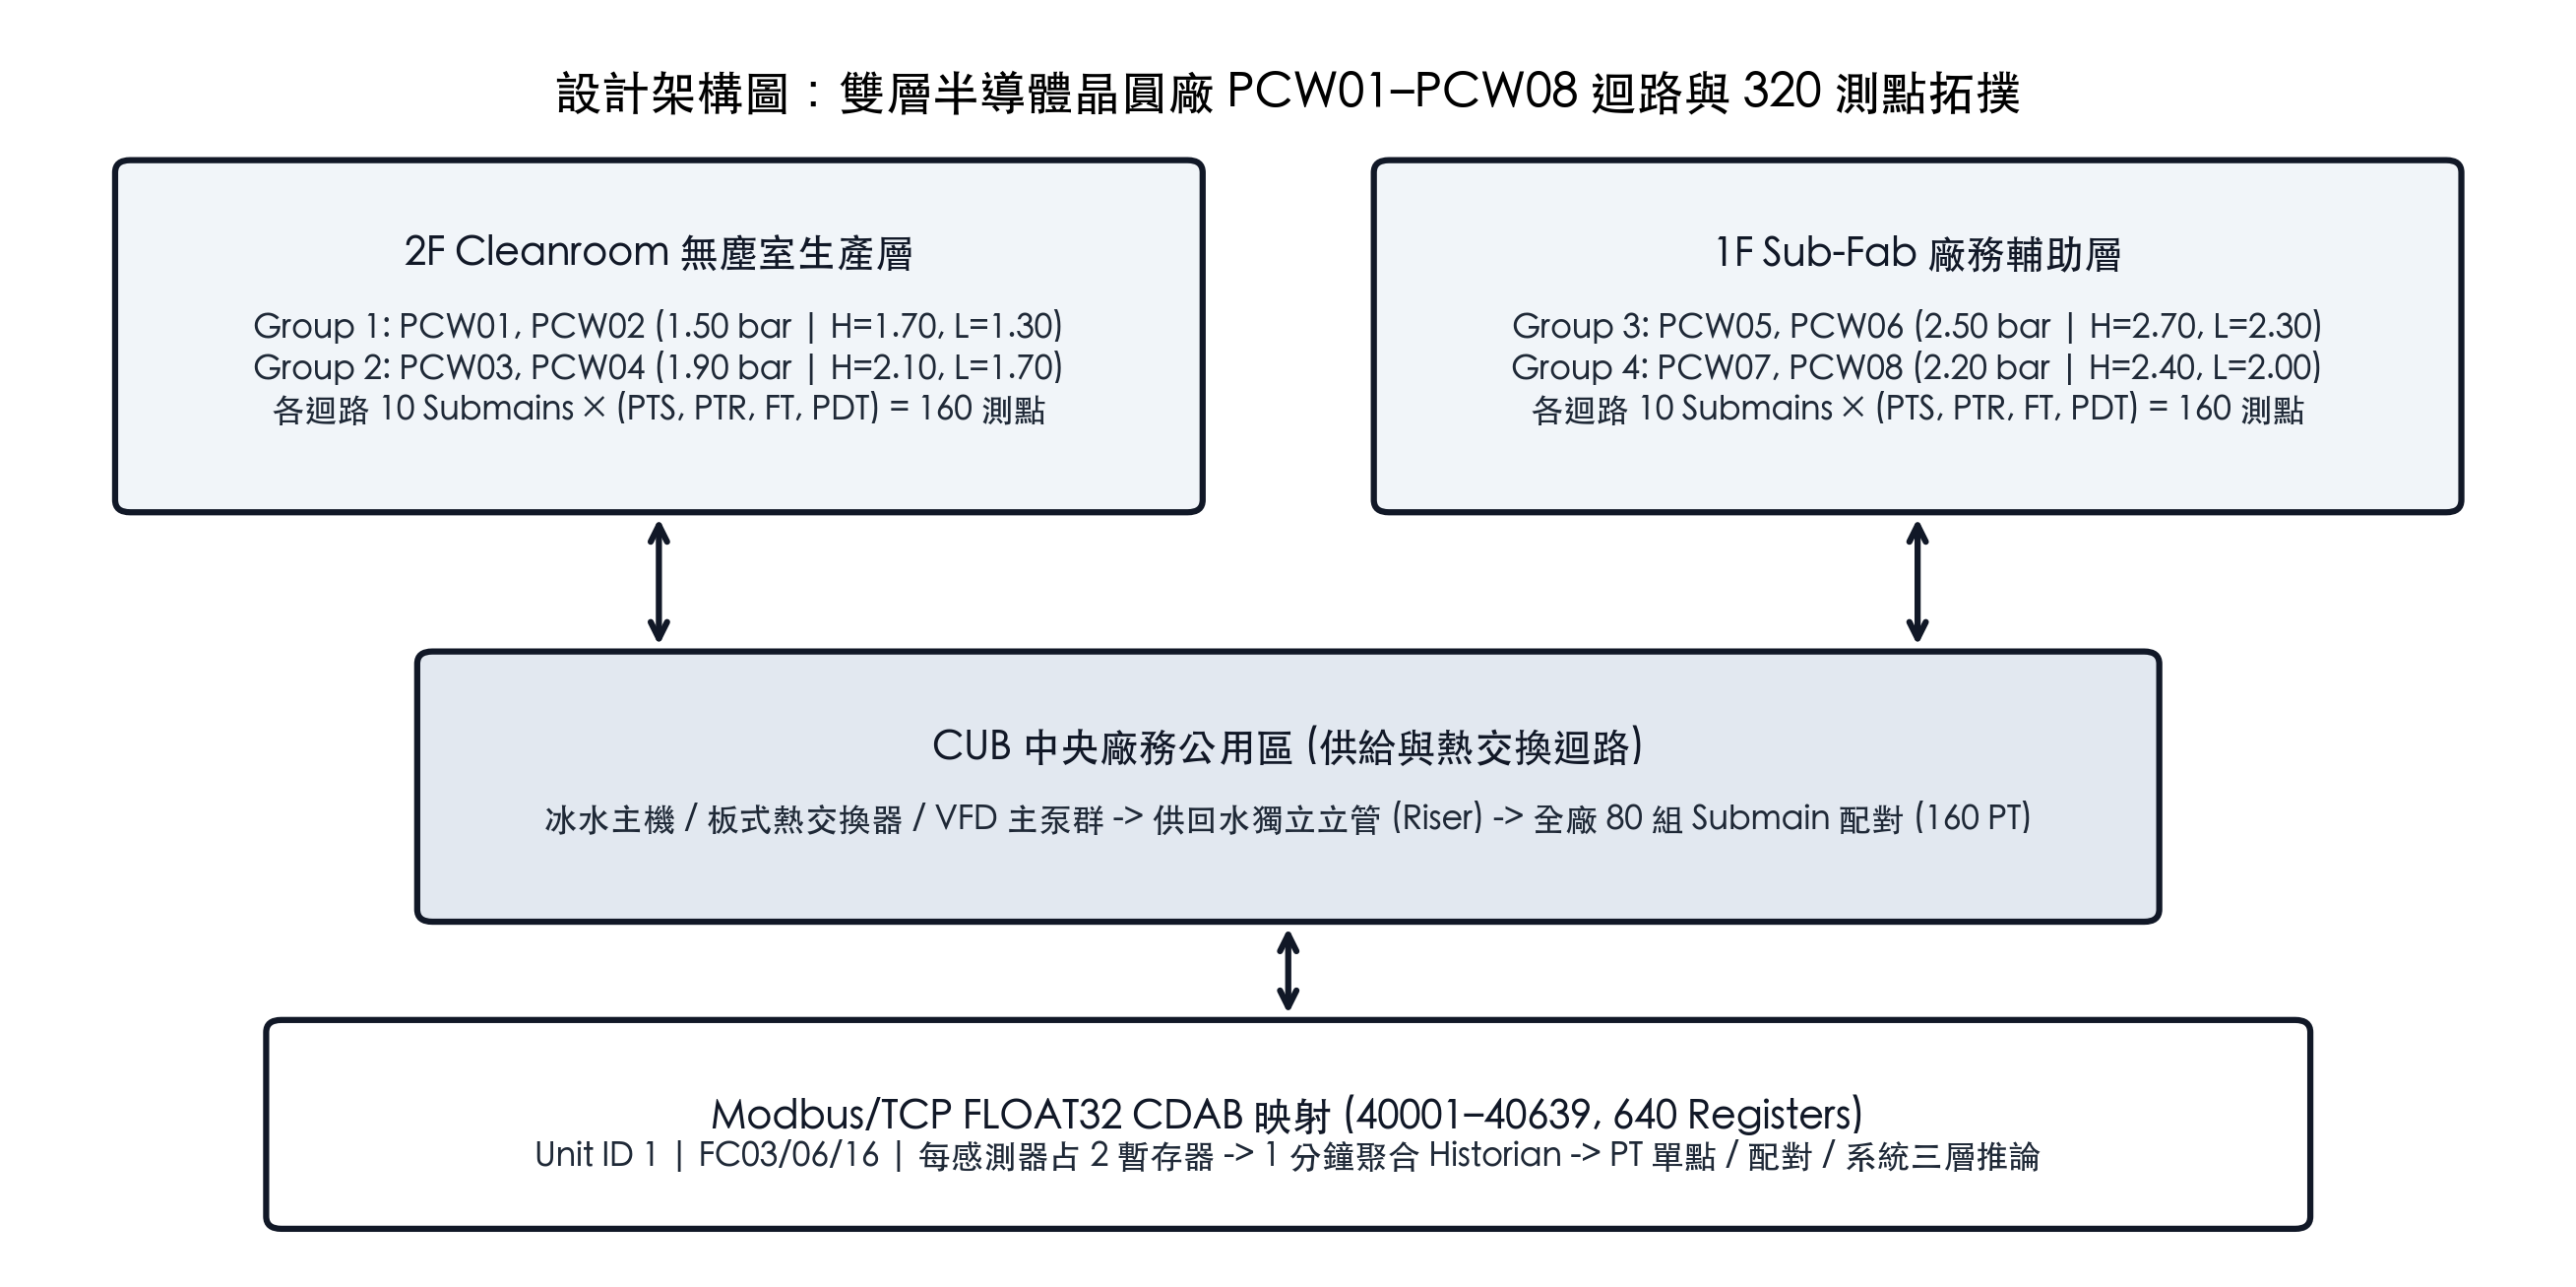
\includegraphics[width=0.92\textwidth,keepaspectratio]{picture/fig_fab_topology_design.png}
    \caption{設計架構圖：雙層晶圓廠 PCW01–PCW08 迴路與 320 測點拓撲配置}
    \label{fig:fab_topo}
\end{figure}

依系統正式設定檔與現場模擬配置，全廠共計 8 套獨立迴路（PCW01 至 PCW08），每套迴路轄下 10 組次幹管（Submain01 至 Submain10），合計 80 組供／回水配對。每組次幹管依標準儀控規格配置 4 支測點：供水壓力計（\texttt{PTS}）、供水流量計（\texttt{FT}）、回水壓力計（\texttt{PTR}）與供回水壓差計（\texttt{PDT}），全廠總計 \textbf{320 支感測器}（包含 \textbf{160 支 PT}、80 支 FT 及 80 支 PDT）。各迴路依設計壓力分屬四大參數分組（Group 1–4），其工程基準與四級安全上下限如表~\ref{tab:pcw_groups_v2} 所示。須特別說明，舊版文件曾將 Group 4 基準誤載為 $2.10\ \mathrm{bar}$ 並虛列溫度計點數，本研究於 Phase 1 程式碼稽核後已統一以系統實作與線上部署之 $2.20\ \mathrm{bar}$ 及 320 測點規格為唯一基準。

\begin{table}[H]
\centering
\caption{PCW 八套獨立迴路四大參數分組基準線與工程安全限值配置表}
\label{tab:pcw_groups_v2}
\footnotesize
\renewcommand{\arraystretch}{1.15}
\setlength{\tabcolsep}{5pt}
\begin{tabularx}{0.98\textwidth}{ccccccc}
\toprule
\textbf{分組代碼} & \textbf{涵蓋迴路} & \textbf{配置樓層} & \textbf{測點類型} & \textbf{Baseline} & \textbf{LoLo / Lo} & \textbf{Hi / HiHi} \\
\midrule
Group 1 & PCW01, PCW02 & 2F Cleanroom & PT (\texttt{PTS}/\texttt{PTR}) & 1.50 bar & 1.20 / 1.30 & 1.70 / 1.80 \\
Group 2 & PCW03, PCW04 & 2F Cleanroom & PT (\texttt{PTS}/\texttt{PTR}) & 1.90 bar & 1.50 / 1.70 & 2.10 / 2.20 \\
Group 3 & PCW05, PCW06 & 1F Sub-Fab   & PT (\texttt{PTS}/\texttt{PTR}) & 2.50 bar & 2.20 / 2.30 & 2.70 / 2.80 \\
Group 4 & PCW07, PCW08 & 1F Sub-Fab   & PT (\texttt{PTS}/\texttt{PTR}) & 2.20 bar & 1.90 / 2.00 & 2.40 / 2.50 \\
\midrule
Group 1/2 & PCW01–04 & 2F Cleanroom & FT (流量) & 180 LPM & 150 / 160 & 200 / 220 \\
Group 3   & PCW05–06 & 1F Sub-Fab   & FT (流量) & 260 LPM & 230 / 240 & 280 / 300 \\
Group 4   & PCW07–08 & 1F Sub-Fab   & FT (流量) & 240 LPM & 200 / 220 & 260 / 280 \\
All       & PCW01–08 & 1F / 2F      & PDT (壓差) & 0.30 bar & 0.00 / 0.10 & 0.50 / 0.60 \\
\bottomrule
\end{tabularx}
\end{table}

\subsection{研究動機、固定門檻侷限與研究目的}
工業 SCADA 系統長期採用固定工程上下限（HI/HIHI/LO/LOLO）作為主要警報機制。固定門檻具備規則明確、易於查核之優點，但在實務監控上存在兩項關鍵缺口：其一，警報觸發當下數值已越過安全邊界，操作人員缺乏事前防禦提前量；其二，當管路因濾網漸進阻塞或閥件微幅異常而產生未越限之持續性行為偏移時，靜態門檻無法發出早期警示，而傳統統計管制圖（如 EWMA）在負載波動下容易累積誤報且無法直接換算剩餘反應時間。須釐清的是，PCW 供水與回水各自具備獨立主管形成封閉循環迴路，異常診斷應依管網壓差與測點行為趨勢判讀，不應以「供回水搶水」作為物理假設。

本研究定位為 \textbf{V1 統計式早期預警方法}，提出下列四項可由實驗逐一檢驗之研究目的：
\begin{enumerate}
    \item 以獲指導教授認可設計方向與準確率之 Excel 初版參考驗證模型為程式開發基礎，嚴格定義\textbf{偏移偵測（Drift Detection）}與\textbf{趨勢預測（Trend Forecast）}兩大核心問題之完整數學公式，遵守 Past-Only 因果約束，並修正既有系統之 $N_{10}$ 不可達盲區與長時段行為偏移失效缺陷。
    \item 實現單一權威規格（Single Source of Truth），使 Excel 參考模型、Python 後端推論引擎與 TypeScript Web SCADA 前端計算結果完全一致。
    \item 實作 Modbus/TCP FLOAT32 CDAB 工業通訊協定伺服器、SQLite 持久化歷史庫與全感測器預警記錄鏈路，修復線上部署版之狀態不同步問題。
    \item 透過 3,840 場受控故障注入、480 筆歷史回放、消融敏感度實驗，以及超過 10 分鐘（11.5 分鐘）真實時序 Modbus 基準行為偏差瀏覽器自動實測，完整量化模型效能、邊界限制與可重現性。
\end{enumerate}

% ============================================================
% 第二章 文獻探討與理論基礎
% ============================================================
\clearpage
\section{文獻探討與理論基礎}

\subsection{工業警報管理標準與預警事件分離}
ANSI/ISA-18.2 規範明確指出，工業警報系統不應僅為靜態越限提示，而須具備明確之狀態生命週期（Active/Unacknowledged、Acknowledged、Cleared、Shelved）、死區（Deadband）與延遲防抖（On-Delay）設計，以避免操作人員遭遇警報疲勞~\cite{isa1822016}。依此原則，本研究將「模型早期預警（T-30 / T-20 / T-10）」與「已越限之硬體工程警報（EVENT / HI / LO）」嚴格分離：前者旨在提供處置緩衝時間，後者代表物理安全界限已被突破。

\subsection{統計製程管制、因果防止洩漏與水力工程先驗}
統計製程管制（SPC）中之指數加權移動平均（EWMA）由 Roberts~\cite{roberts1959control} 提出並廣泛整理於 Montgomery~\cite{montgomery2020statistical}，其藉由指數衰減權重提高對微小平均偏移之偵測靈敏度。然而 EWMA 僅輸出無因次控制統計量，不直接提供物理單位之外推到限時間，且在非定常工業負載下易受基準漂移影響而升高誤報率。

在時序預測與異常偵測建模中，Kaufman 等人~\cite{kaufman2012leakage} 指出任何使用評估時刻之後資訊的特徵計算皆屬資料洩漏（Data Leakage），將導致離線驗證效能虛高卻無法於線上重現。因此本研究嚴格要求所有基準統計量與斜率估計均限制在過去半開區間 $[t-W, t)$ 內執行。此外，Darcy~\cite{darcy1857recherches} 與 Colebrook~\cite{colebrook1939turbulent} 所奠定之管流摩擦壓降與雷諾數關係式，說明穩態下壓差與流量變化之工程物理意義，本研究將其作為供回水配對診斷之工程先驗背景；然因現場未量測各支管粗糙度與等效管長，模型本體仍保持純統計時序推論，不虛構未經校準之物理數位分身。

在資料通訊協定層面，本系統後端伺服器依循 Modbus Organization 官方規範~\cite{modbus2006spec} 實作 Modbus/TCP MBAP 訊框與 Holding Registers（FC03/FC06/FC16）雙向讀寫機制。

% ============================================================
% 第三章 系統架構與統計式早期預警方法
% ============================================================
\clearpage
\section{系統架構與統計式早期預警方法}

\subsection{五層式軟硬體架構與實作邊界}
如圖~\ref{fig:arch_layers} 所示，本研究重構之系統採五層分層架構，明確區分「已實作並完成實機驗證之元件（實線）」與「需廠務授權串接之規劃項目（虛線）」。與舊版僅存瀏覽器端記憶體模擬器之原型不同，重構後系統於後端整合純 Python 非同步 Modbus/TCP 伺服器（Port 15020）、SQLite WAL 歷史與預警執行紀錄資料庫、統一推論／警報引擎，以及 FastAPI REST/WebSocket 介面，並透過瀏覽器實時渲染 9 大 Web SCADA 頁面。

\begin{figure}[H]
    \centering
    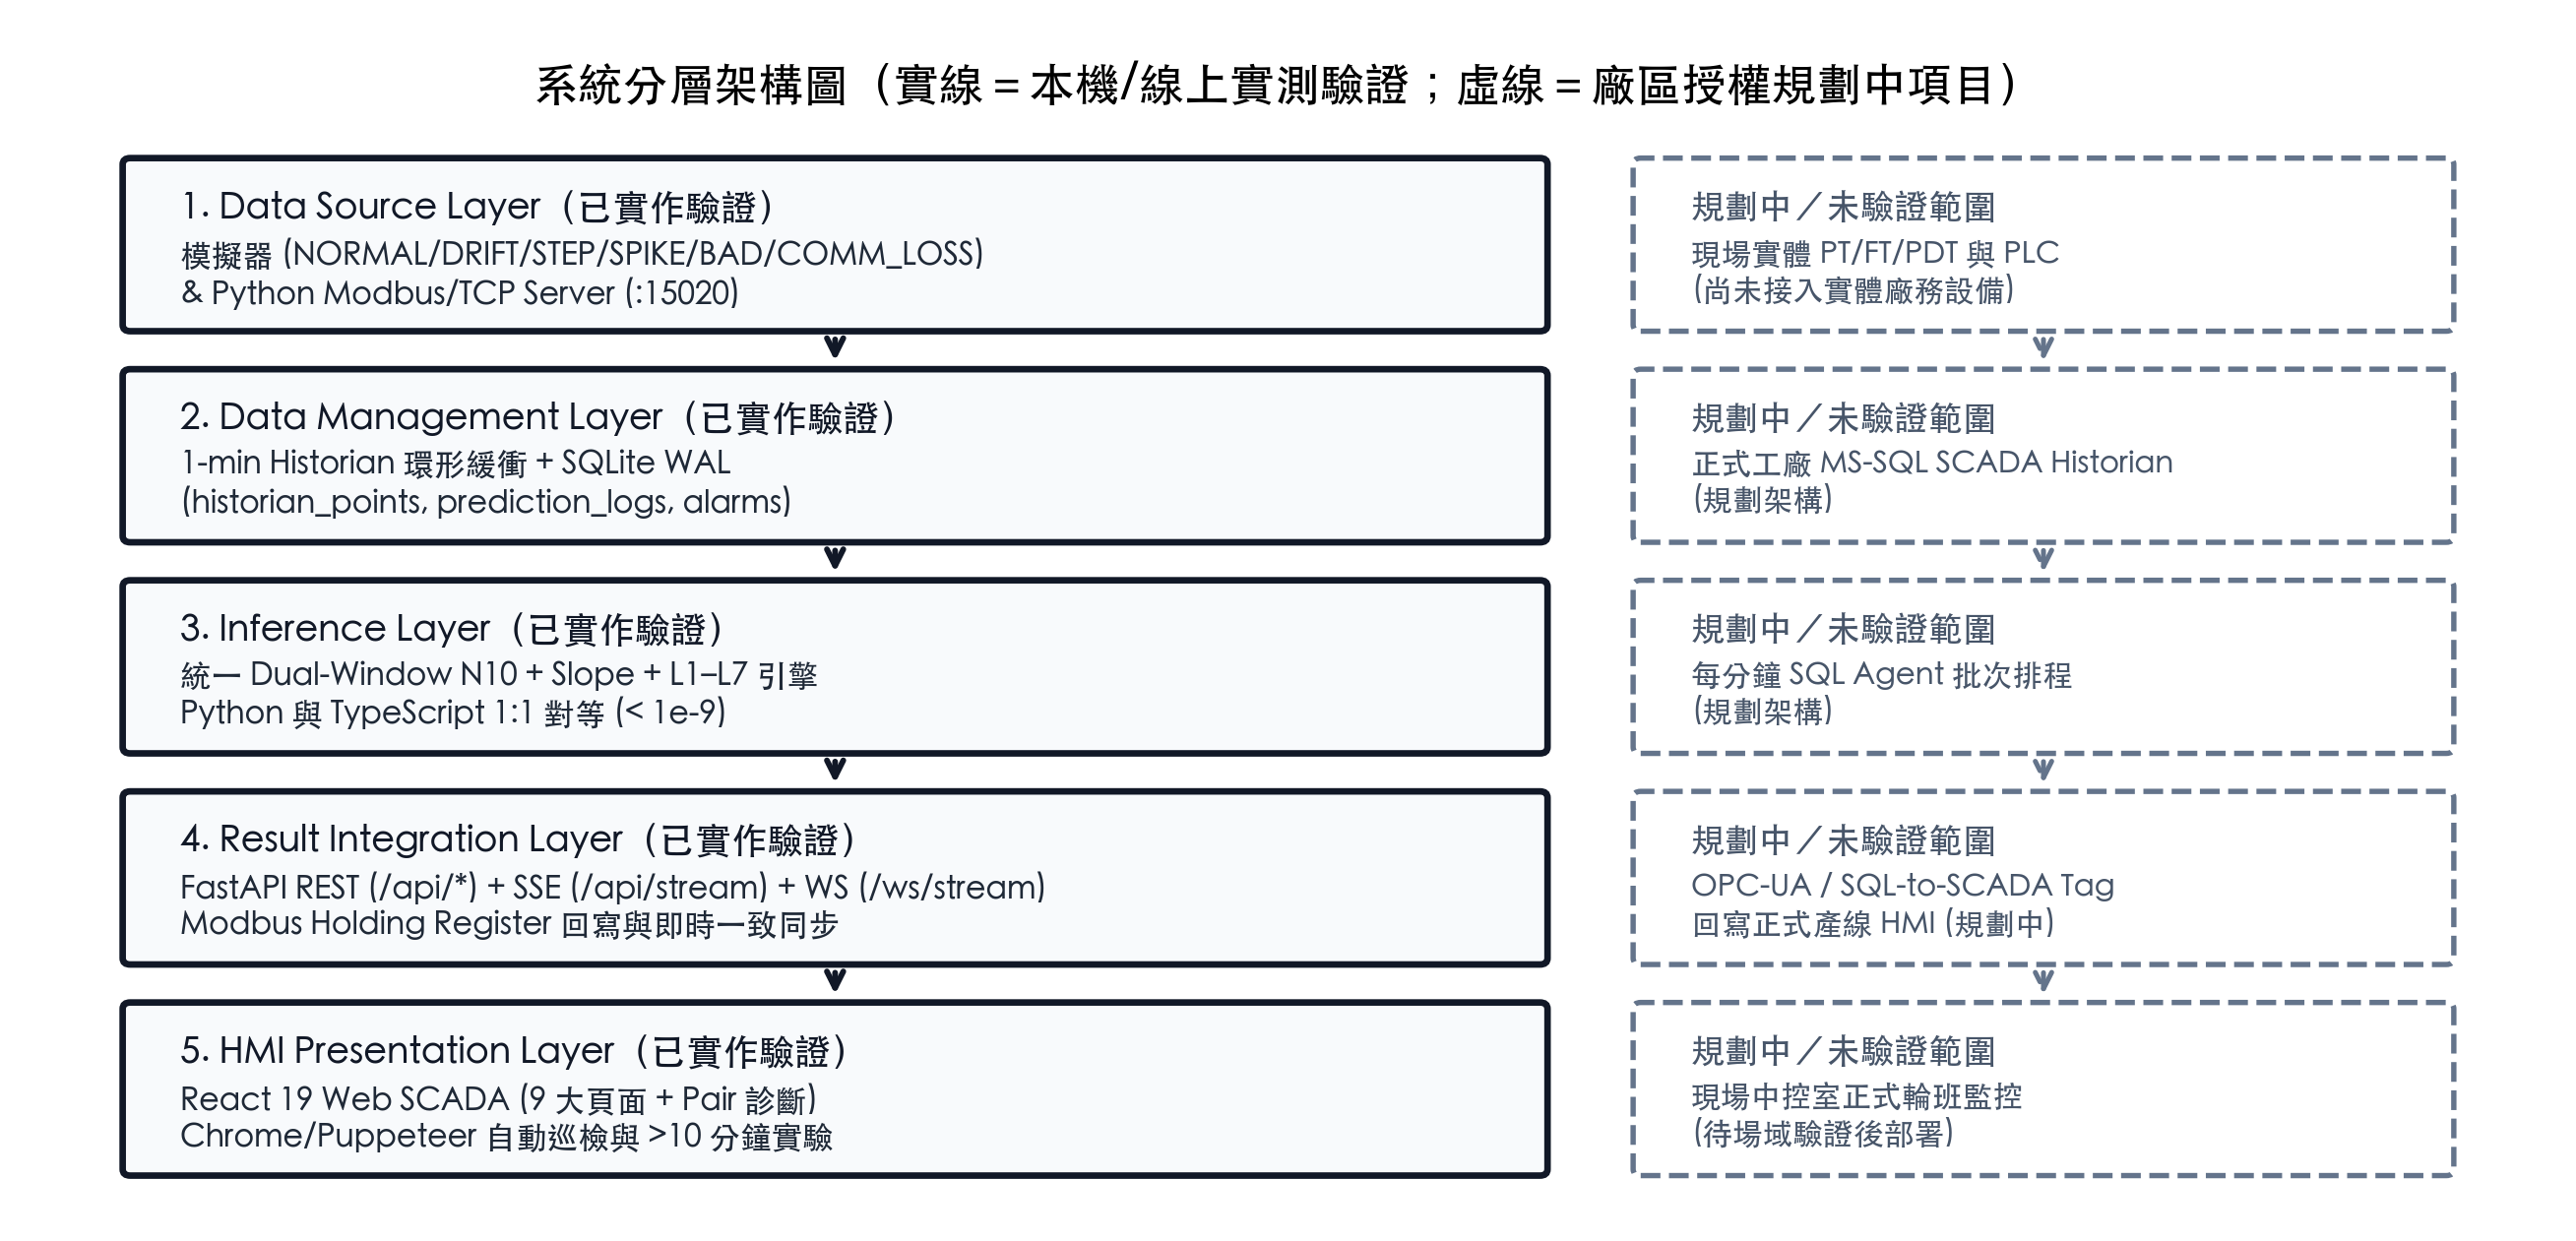
\includegraphics[width=0.95\textwidth,keepaspectratio]{picture/fig_system_architecture_layers.png}
    \caption{五層式系統架構與已實作驗證／規劃中元件邊界圖}
    \label{fig:arch_layers}
\end{figure}

\subsection{Modbus/TCP 暫存器映射與 1 分鐘時序聚合}
全廠 320 個測點依表~\ref{tab:modbus_map_v2} 連續映射至 Modbus Holding Registers \texttt{40001} 至 \texttt{40639}（共 640 個 16-bit 暫存器）。每個測點採用 IEEE-754 單精度浮點數（FLOAT32）配合 CDAB Word-Swap 位元組順序，將工程物理值無失真編碼為相鄰兩個暫存器。系統高頻採樣（預設 $1\ \mathrm{Hz}$）於每分鐘邊界聚合所有品質為 \texttt{GOOD} 之樣本算術平均寫入 Historian；若該分鐘 \texttt{GOOD} 樣本比例低於 $50\%$，則標記為 \texttt{BAD} 或 \texttt{COMM\_LOSS}。

\begin{table}[H]
\centering
\caption{全廠 320 測點 Modbus/TCP FLOAT32 (CDAB) 保持暫存器位址映射表}
\label{tab:modbus_map_v2}
\footnotesize
\renewcommand{\arraystretch}{1.15}
\setlength{\tabcolsep}{4pt}
\begin{tabularx}{\textwidth}{cccXc}
\toprule
\textbf{迴路} & \textbf{暫存器位址} & \textbf{Submain} & \textbf{涵蓋測點與數量} & \textbf{編碼格式} \\
\midrule
PCW01 & 40001 -- 40079 & Submain01--10 & 20 PT, 10 FT, 10 PDT (40 點) & FLOAT32 CDAB \\
PCW02 & 40081 -- 40159 & Submain01--10 & 20 PT, 10 FT, 10 PDT (40 點) & FLOAT32 CDAB \\
PCW03 & 40161 -- 40239 & Submain01--10 & 20 PT, 10 FT, 10 PDT (40 點) & FLOAT32 CDAB \\
PCW04 & 40241 -- 40319 & Submain01--10 & 20 PT, 10 FT, 10 PDT (40 點) & FLOAT32 CDAB \\
PCW05 & 40321 -- 40399 & Submain01--10 & 20 PT, 10 FT, 10 PDT (40 點) & FLOAT32 CDAB \\
PCW06 & 40401 -- 40479 & Submain01--10 & 20 PT, 10 FT, 10 PDT (40 點) & FLOAT32 CDAB \\
PCW07 & 40481 -- 40559 & Submain01--10 & 20 PT, 10 FT, 10 PDT (40 點) & FLOAT32 CDAB \\
PCW08 & 40561 -- 40639 & Submain01--10 & 20 PT, 10 FT, 10 PDT (40 點) & FLOAT32 CDAB \\
\bottomrule
\end{tabularx}
\end{table}

\subsection{Excel 初版參考模型設計基礎與 Past-Only 因果視窗}
本研究之演算法設計以獲指導教授認可設計方向與準確率之初版 Excel 驗證工作簿（\texttt{PCW\_T30\_T20\_T10\_FINAL\_ROLLBACK\_THESIS\_VERIFICATION.xlsx}）為程式開發基礎。該工作簿於 \texttt{Parameters}、\texttt{MinuteInference} 與 \texttt{Thesis\_Model} 工作表中確立了系統欲解決之兩大核心數學問題——\textbf{偏移偵測（Drift Detection）}與\textbf{趨勢預測（Trend Forecast）}，並將「即時推論欄位（僅看過去，\texttt{Pred\_T30/T20/T10}）」與「離線驗收欄位（可看未來驗證，\texttt{Actual\_T30/T20/T10}）」完全隔離，保證絕無未來資料洩漏（Past-Only）。初版 Excel 凍結參數包含：警報界限 $L_{\mathrm{alarm}} = 1.70\ \mathrm{bar}$、密度門檻 $\theta = 2$、趨勢窗長 $5\ \mathrm{min}$、基準窗長 $60\ \mathrm{min}$、近期窗長 $10\ \mathrm{min}$，以及對應三種預警視域之輔助門檻 $G_{30} = 1.55$、$G_{20} = 1.58$、$G_{10} = 1.62$。

如圖~\ref{fig:window_design} 所示，於推論時刻 $t$，系統僅讀取過去 70 分鐘已結算之歷史資料，並切分為三個互斥區間：
\begin{enumerate}
    \item \textbf{歷史基準區間（60 分鐘）}：範圍 $[t-70, t-10)$，用來建立該感測器近期穩態的「正常參考基準線」。
    \item \textbf{前期局部區間（5 分鐘）}：範圍 $[t-10, t-5)$，作為計算近期變化斜率的起點平均值（$\mathrm{Prev5Avg}$）。
    \item \textbf{近期局部區間（5 分鐘）}：範圍 $[t-5, t)$，作為計算近期變化斜率的終點平均值（$\mathrm{Recent5Avg}$）；將上述前後兩段 5 分鐘合併即為\textbf{近期 10 分鐘觀察區間} $[t-10, t)$。
\end{enumerate}
表~\ref{tab:excel_to_program_map} 以直觀對照方式彙整 Excel 每一欄位與本系統 \textbf{Unified V1} 程式實作之間的數學對應。

\begin{figure}[H]
    \centering
    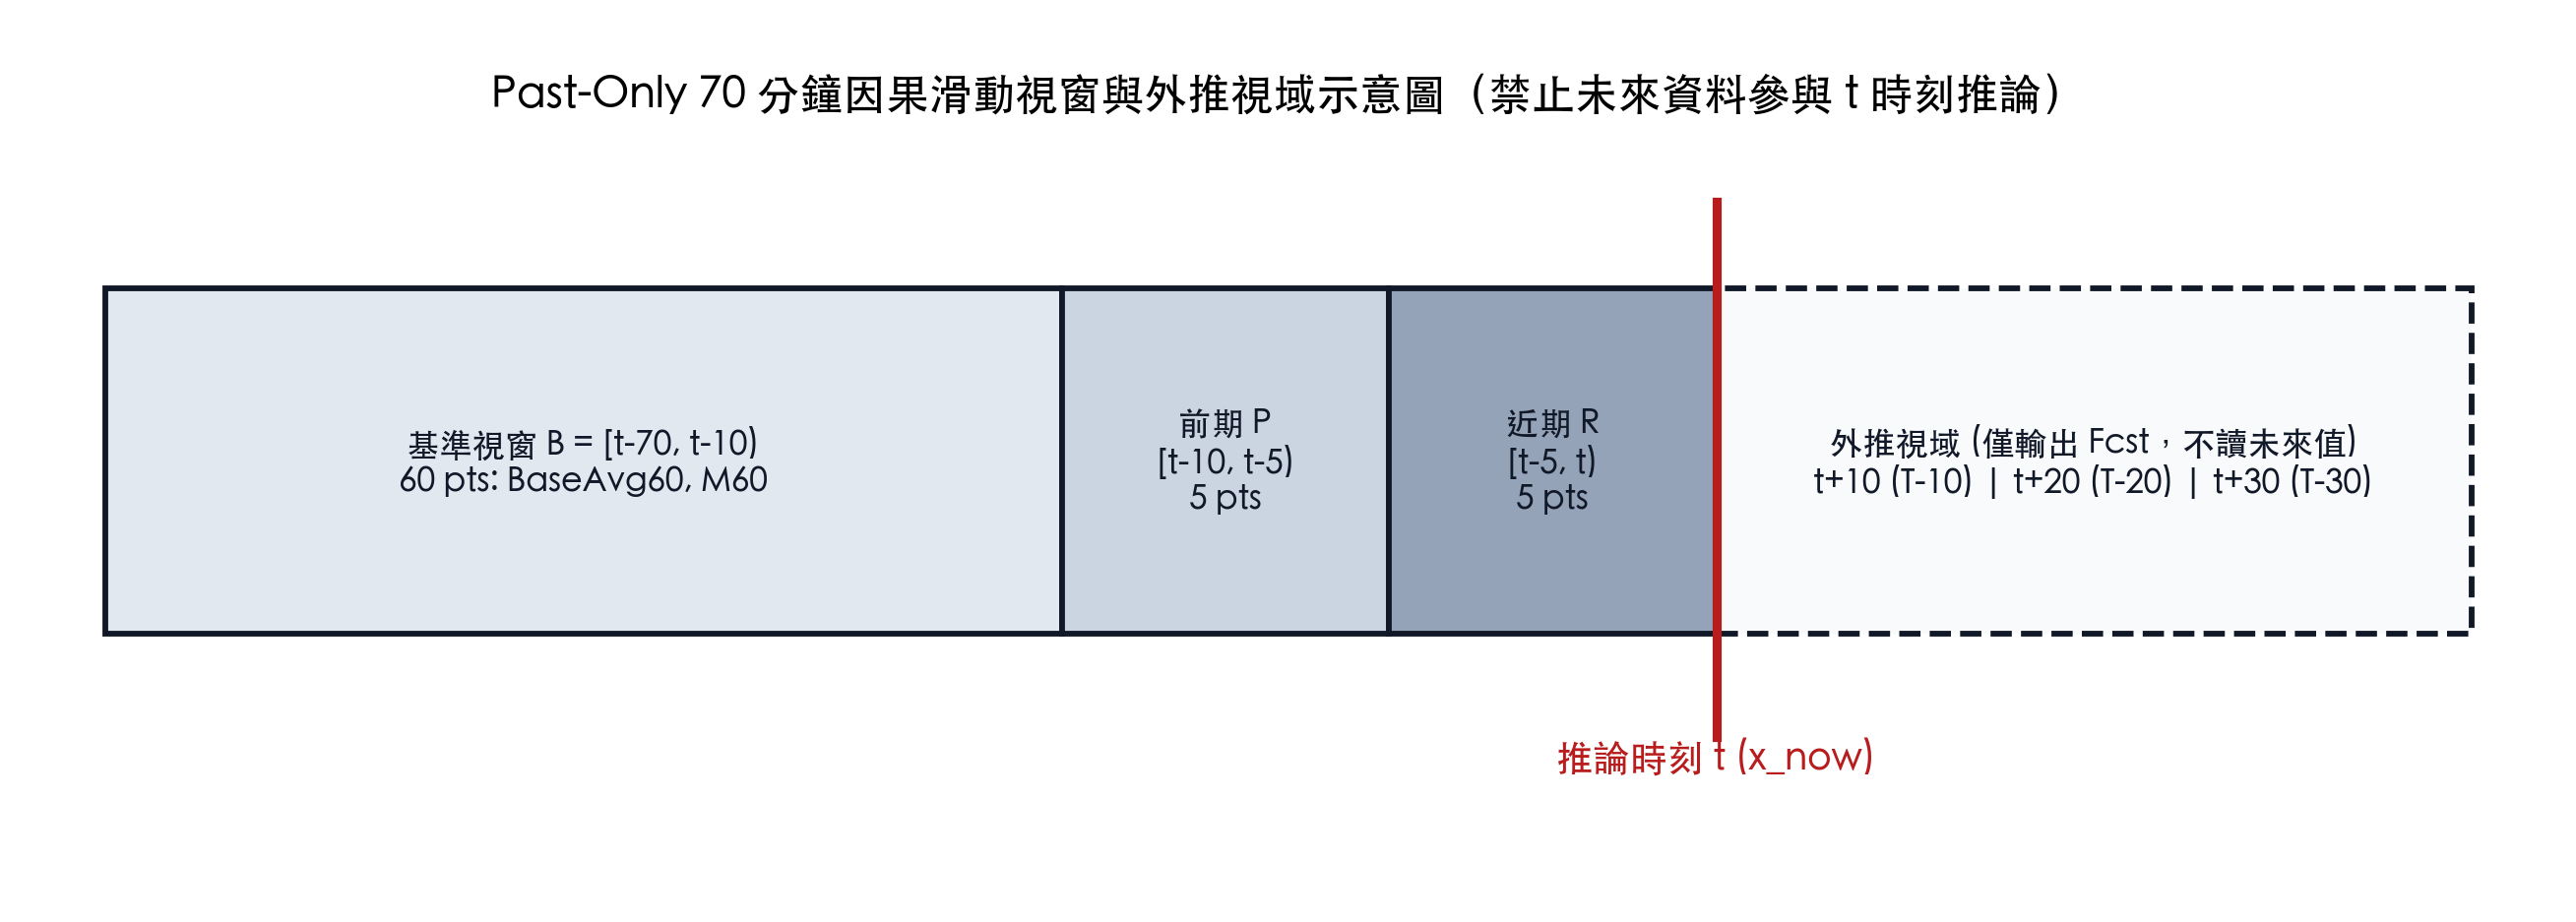
\includegraphics[width=0.92\textwidth,keepaspectratio]{picture/fig_past_only_window_design.png}
    \caption{Past-Only 70 分鐘因果滑動視窗切分與多視域外推示意圖}
    \label{fig:window_design}
\end{figure}

\begin{table}[H]
\centering
\caption{Excel 初版參考模型（\texttt{MinuteInference}）至重構系統 Unified V1 簡明公式對照表}
\label{tab:excel_to_program_map}
\scriptsize
\renewcommand{\arraystretch}{1.2}
\setlength{\tabcolsep}{3.5pt}
\begin{tabularx}{\textwidth}{>{\bfseries}l l X X}
\toprule
問題歸屬 & Excel 欄位 / 參數 & Excel 初版公式（單向上漂） & 程式重構 Unified V1 公式（雙向 / 全廠 320 點） \\
\midrule
事件界限 & \texttt{D4} / \texttt{AlarmLimit} & 讀值 $\ge 1.70$ 即為 \texttt{EVENT} & 讀值 $\ge H_i$ 或 $\le L_i$ 即為 \texttt{EVENT}（L5 事件分離） \\
偏移偵測 & \texttt{K4} (\texttt{BaseAvg60}) & 過去 60 分鐘 $[t-70,t-10)$ 平均值 & 同左，但僅計入 \texttt{GOOD} 樣本且至少須 30 點（L1） \\
偏移偵測 & \texttt{L4, M4} (\texttt{M60, M10}) & $60\mathrm{m}/10\mathrm{m}$ 內大於 $B_{60}$ 之筆數 & 依變化方向統計同向偏離筆數並按滿窗比例還原（式~\eqref{eq:m60_m10}） \\
偏移偵測 & \texttt{N4} (\texttt{N10}) & $M_{10} \div (M_{60}/6)$；判定採 $N_{10} > 2$ & 修正為 $N_{10} \ge \theta$（式~\eqref{eq:n10}），避免常態雜訊無法達標 \\
偏移偵測 & \texttt{Gate30/20/10} & 當前值需達 $\{1.55,1.58,1.62\}$ & 改為跨度比例門檻 $\ge g\%\times(H_i-L_i)$（式~\eqref{eq:drift_gate}） \\
趨勢預測 & \texttt{E4, F4} (\texttt{Prev5, Recent5}) & $[t-10,t-5)$ 與 $[t-5,t)$ 平均 & 同左，僅計算 \texttt{GOOD} 品質樣本之算術平均 \\
趨勢預測 & \texttt{G4} (\texttt{Slope/min}) & $\max\bigl(0,\; (\mathrm{Recent5}-\mathrm{Prev5})\div 5\bigr)$ & 保留正負號 $(\mathrm{Recent5}-\mathrm{Prev5})\div 5$（式~\eqref{eq:base_slope}） \\
趨勢預測 & \texttt{H4:J4} (\texttt{Forecast30/20/10}) & 目前值 $+$ 斜率 $\times\ h$ 分鐘 & 雙向外推 $+$ 近 10 點回歸信賴區間 $+$ 到限時間 $\mathrm{TTL}$ \\
聯合決策 & \texttt{O4:Q4, W4} (\texttt{Pred\_T*}) & （外推觸限）或（$N_{10}>2$ 且達 Gate） & （外推觸限）或（偏移成立）$+$ 防抖鎖存（L6） \\
\bottomrule
\end{tabularx}
\end{table}

\noindent\textbf{【口試備註：為何固定切 60 分鐘基準與 10 分鐘近期，不看即時那 1 分鐘？】}\\
因為嚴格規定只用「過去已經完成」的 70 分鐘資料推論現在，就像考試時不准偷看未來答案；60 分鐘夠長可代表穩態常規，而前後兩段 5 分鐘平均可以濾除單點雜訊跳動。

\subsection{核心模型一：偏移偵測數學公式 (Drift Detection Model)}
\label{sec:drift_detection}
偏移偵測模型旨在解決：「數值還沒撞到固定警報線（如 $1.70\ \mathrm{bar}$），但已經明顯比過去一小時常態平均更常偏高（或偏低）且持續維持不退」之異常行為辨識。

\subsubsection{Excel 初版雙視窗異常密度基礎公式}
在 Excel 工作簿（\texttt{MinuteInference!K:N}）中，偏移偵測分成直覺的三步驟：
\begin{align}
\mathrm{BaseAvg}_{60}(t) &= \text{過去 60 分鐘 } [t-70, t-10) \text{ 資料之算術平均值} \nonumber \\
M_{60}^{\mathrm{XL}}(t) &= \text{過去 60 分鐘內，大於 } \mathrm{BaseAvg}_{60}(t) \text{ 之筆數} \nonumber \\
M_{10}^{\mathrm{XL}}(t) &= \text{最近 10 分鐘內，大於 } \mathrm{BaseAvg}_{60}(t) \text{ 之筆數}
\label{eq:excel_drift_counts}
\end{align}
接著比較「近 10 分鐘異常密度」是「過去 60 分鐘常態密度」的幾倍（因為 60 分鐘是 10 分鐘的 6 倍，常態期望值為 $M_{60}/6$），並搭配分段輔助門檻 $G_h \in \{1.55, 1.58, 1.62\}$ 確認水位已開始上升：
\begin{align}
N_{10}^{\mathrm{XL}}(t) &= \begin{cases}
\dfrac{M_{10}^{\mathrm{XL}}(t)}{M_{60}^{\mathrm{XL}}(t) \div 6}, & \text{當 } M_{60}^{\mathrm{XL}}(t) > 0 \\[8pt]
999, & \text{當 } M_{60}^{\mathrm{XL}}(t)=0 \text{ 且 } M_{10}^{\mathrm{XL}}(t)>0 \\
0, & \text{當 } M_{60}^{\mathrm{XL}}(t)=0 \text{ 且 } M_{10}^{\mathrm{XL}}(t)=0
\end{cases} \nonumber \\
\text{Excel 偏移證據成立} &\iff \bigl(N_{10}^{\mathrm{XL}}(t) > 2\bigr) \;\text{且}\; \bigl(x(t) \ge G_h\bigr) \qquad (h\in\{30,20,10\})
\label{eq:excel_n10}
\end{align}

\noindent\textbf{【口試備註：分母為什麼要除以 6？$N_{10} > 2$ 代表什麼意思？】}\\
口試簡答：「因為基準窗是 60 分鐘，近期窗是 10 分鐘，時間長度差 6 倍！把 $M_{60}$ 除以 6，就換算成『平均每 10 分鐘應該要有幾次偏高』。舉例來說，若過去平均每 10 分鐘只有 3 筆偏高，但最近 10 分鐘卻出現 8 筆偏高，那 $N_{10} = 8 \div 3 = 2.67$ 倍，超過 2 倍門檻就代表行為明顯偏離常態了。若歷史全在平均以下（$M_{60}=0$），則用 999 代表密度暴增極端值。」

\subsubsection{程式化泛化、對稱雜訊盲區修正與持續水準偏移閘門}
將 Excel 公式搬移到全廠 320 支感測器（涵蓋 PT/FT/PDT）並連續運行超過 10 分鐘時，程式實作保留上述「$N_{10}$ 密度倍率」核心，僅作四項必要且直白的工程補強：

\textbf{（1）Layer 1 品質檢查：}只計入品質標記為 \texttt{GOOD} 的資料點。若過去 70 分鐘內有效點比例低於 $80\%$、基準期不滿 30 點，或兩個 5 分鐘局部窗任一段缺點，系統立即停機保護並回報 \texttt{INSUFFICIENT\_DATA}。

\textbf{（2）支援雙向偏離與缺測比例還原：}PCW 除了壓力異常爬高，管線破裂或阻斷也可能讓壓力／流量往下掉。程式依據變化斜率方向決定檢查「高於基準」或「低於基準」，並在發生少量缺測時按滿窗長度（60 與 10）等比例縮放還原後四捨五入：
\begin{align}
M_{60}(t) &= \mathrm{round}\!\left(\text{基準區間同向偏離個數} \times \frac{60}{\text{基準有效點數}}\right) \nonumber \\
M_{10}(t) &= \mathrm{round}\!\left(\text{近 10 分區間同向偏離個數} \times \frac{10}{\text{近期有效點數}}\right)
\label{eq:m60_m10}
\end{align}
無因次密度倍率公式與 Excel 式~\eqref{eq:excel_n10} 完全一致：
\begin{equation}
N_{10}(t) = \begin{cases}
\dfrac{M_{10}(t)}{M_{60}(t) \div 6}, & \text{當 } M_{60}(t) > 0 \\[8pt]
999, & \text{當 } M_{60}(t)=0 \text{ 且 } M_{10}(t)>0 \\
0, & \text{當 } M_{60}(t)=0 \text{ 且 } M_{10}(t)=0
\end{cases}
\label{eq:n10}
\end{equation}

\textbf{（3）修正盲區與 Layer 2 跨度水準偏移雙重保護：}將 Excel 的固定門檻 $G_h$ 改寫為通用所有感測器的「操作跨度比例門檻」，令各測點正常跨度 $S_i = H_i - L_i$、近期與基準的水準差距 $\Delta\mu_{10}(t) = |\mathrm{Avg}_{10}(t) - \mathrm{BaseAvg}_{60}(t)|$，定義最終偏移偵測成立條件為：
\begin{equation}
\text{偏移偵測成立} \iff \bigl(N_{10}(t) \ge \theta\bigr) \;\text{且}\; \Bigl(|\mathrm{Slope}(t)\times 30| \ge \frac{g}{100}S_i \;\text{或}\; \Delta\mu_{10}(t) \ge \frac{g}{100}S_i\Bigr)
\label{eq:drift_gate}
\end{equation}
預設靈敏度 $\theta = 2.0$、跨度門檻百分比 $g = 5.0\%$（例如 Group 1 PT 跨度 $1.70 - 1.30 = 0.40\ \mathrm{bar}$，其 $5\%$ 即為 $0.02\ \mathrm{bar}$）。

\noindent\textbf{【口試備註：程式相對 Excel 到底改修了哪兩件關鍵大事？（高機率必問！）】}
\begin{enumerate}
    \item \textbf{為什麼把 $N_{10} > 2$ 改成 $N_{10} \ge 2$？} 當常態雜訊剛好一半以上落在均值上方時（$M_{60} \ge 30$），就算最近 10 分鐘「全數 10 筆都異常」（$M_{10}=10$），算出來最大值也只有 $10 \div (30/6) = 2.0$，寫大於 `>` 會讓這個門檻在數學上永遠不可能達到，改成大於等於 `>=` 就徹底修復此盲區。
    \item \textbf{為什麼多加了 $|\mathrm{Avg}_{10} - \mathrm{BaseAvg}_{60}|$ 這一項？} 當把 Modbus 基準拉高維持超過 10 分鐘後，最近 10 分鐘全部都在高檔，前 5 分鐘和後 5 分鐘平均值相同，斜率會掉回接近 $0$。如果不看近期平均和歷史基準平均的「水準高度差」，超過 10 分鐘預警就會誤解除；加上這一項才能在實測中穩穩持續抓到異常！
\end{enumerate}

\subsection{核心模型二：趨勢預測數學公式 (Trend Forecast Model) 與七層工業硬化}
\label{sec:trend_forecast}
趨勢預測模型旨在解決：「在目前還沒越線前，以現在的變化速度推估，10 / 20 / 30 分鐘後是否會撞線？大概還剩幾分鐘反應時間？預測的信心範圍有多寬？」

\subsubsection{Excel 初版局部斜率與多視域外推基礎公式}
為避免對前後兩分鐘直接相減造成斜率過度劇烈震盪，Excel 模型（\texttt{MinuteInference!E:J}）先計算前 5 分鐘與近 5 分鐘的兩個平均值，再求每分鐘變化速度（$\mathrm{Slope}$）並線性外推未來 $h \in \{30, 20, 10\}$ 分鐘數值：
\begin{equation}
\mathrm{Prev5Avg}(t) = \text{區間 } [t-10, t-5) \text{ 之平均}, \qquad
\mathrm{Recent5Avg}(t) = \text{區間 } [t-5, t) \text{ 之平均}
\label{eq:excel_5m_avgs}
\end{equation}
\begin{align}
\mathrm{Slope}_{\mathrm{XL}}(t) &= \max\!\left(0,\; \frac{\mathrm{Recent5Avg}(t) - \mathrm{Prev5Avg}(t)}{5}\right) \nonumber \\
\mathrm{Forecast}_{h}^{\mathrm{XL}}(t) &= x(t) + \mathrm{Slope}_{\mathrm{XL}}(t) \times h \qquad (h \in \{30, 20, 10\})
\label{eq:excel_forecast}
\end{align}
於決策端（\texttt{MinuteInference!D, O:Q, W}），只要當前還沒觸及固定警報（$x(t) < 1.70$），Excel 同時檢查「趨勢外推觸線」或「偏移密度達標」兩條路（取聯集 \textbf{OR}）：
\begin{equation}
\begin{split}
\text{發出 } T\text{-}h\text{ 預警} \iff &\text{目前尚未越界 } (x(t) < 1.70) \\
&\text{且}\; \Bigl(\mathrm{Forecast}_{h}^{\mathrm{XL}}(t) \ge 1.70 \;\text{或}\; \bigl[N_{10}^{\mathrm{XL}}(t) > 2 \text{ 且 } x(t) \ge G_h\bigr]\Bigr)
\end{split}
\label{eq:excel_pred_rule}
\end{equation}
狀態顯示依緊急順序判定：\texttt{EVENT}（已越界）$\succ$ \texttt{T-10} $\succ$ \texttt{T-20} $\succ$ \texttt{T-30} $\succ$ \texttt{Normal}。

\noindent\textbf{【口試備註：為什麼分母是除以 5？為什麼不直接用兩點相減算斜率？】}\\
因為兩段 5 分鐘窗格的中心點剛好相距 5 分鐘（$[t-10,t-5)$ 中心在 $t-7.5$，$[t-5,t)$ 中心在 $t-2.5$，中心距正好是 5 分鐘），把兩個平均值的高度差除以 5 分鐘，就是平滑後的「每分鐘爬升速率」，既簡單好算、又不容易被單一秒的雜訊帶偏！

\subsubsection{程式化雙向斜率、OLS 95\% 預測區間與閉式 TTL}
程式開發直接承襲上述外推與雙路 OR 結構，並補充四項控制室實用功能：

\textbf{（1）有號雙向基準與局部斜率：}去除 Excel $\max(0,\cdot)$ 截斷，同時計算高限趨近與低限趨近：
\begin{align}
\mathrm{Slope}(t) &= \frac{\mathrm{Recent5Avg}(t) - \mathrm{Prev5Avg}(t)}{5} \nonumber \\
\hat{x}(t+h) &= x_{\mathrm{now}} + \mathrm{Slope}(t) \times h \qquad (h\in\{10,20,30\})
\label{eq:base_slope}
\end{align}
只要 $\hat{x}(t+h) \ge H_i$（上限）或 $\le L_i$（下限）即觸發該視域之預警。

\textbf{（2）Layer 3 近期 10 分鐘回歸線與 95\% 信賴區間（畫面錐形圖）：}為告訴操作員「趨勢線準不準、誤差有多大」，程式對最近 $n=10$ 分鐘點位執行標準線性回歸（OLS），算出最佳擬合直線 $\hat{y}(h) = a + b \cdot h$、配適度指標 $R^2$（越接近 1 代表線性趨勢越明確）與殘差標準差 $s_e$：
\begin{align}
R^2 &= 1 - \frac{\text{模型殘差平方和 (SSE)}}{\text{總變異平方和 (SST)}} \nonumber \\
s_e &= \sqrt{\frac{\text{SSE}}{n - 2}}
\label{eq:ols_fit}
\end{align}
接著套用統計學標準 Student-$t$ 公式（$n=10$ 自由度為 8 時查表乘數 $t_{0.975,8} = 2.306$），算出未來第 $h$ 分鐘的 95\% 不確定性半寬 $\delta_h$，即系統介面上呈現隨時間漸寬的上下誤差錐面（$\hat{y}(h) \pm \delta_h$）：
\begin{equation}
\delta_h = 2.306 \times s_e \times \sqrt{1 + \frac{1}{n} + \text{時間外推距離修正項}}
\label{eq:pred_band}
\end{equation}

\noindent\textbf{【口試備註：OLS 95\% 預測區間這條很長要怎麼跟教授解釋？】}\\
口試不用背根號裡的展開項，直接告訴教授：「前面式~\eqref{eq:base_slope} 的五分鐘平均差負責給出穩定的預測中心線；這條則是用標準教科書的最小平方法（OLS）對近 10 分鐘資料算殘差標準差 $s_e$ 乘上 95\% Student-$t$ 臨界值 $2.306$，讓 Web 畫面能畫出『越往未來 30 分鐘、預測不確定範圍會越寬』的漏斗形風險帶，方便操作員評估可信度。」

\textbf{（3）Layer 4 剩餘到限時間（Time-To-Limit, TTL）：}令 $U^*$ 為當前變化方向上最近尚未跨越之工程警報門檻，沿用直觀的「剩餘距離 $\div$ 目前變化速度」估算還會剩幾分鐘抵達警報門檻（單位：分鐘；若趨於平坦或超過 24 小時則不顯示）：
\begin{equation}
\mathrm{TTL}(t) = \frac{U^* - x_{\mathrm{now}}}{\mathrm{Slope}(t)}
\label{eq:ttl}
\end{equation}

\textbf{（4）Layer 5–7 決策分層、防抖鎖存與風險評分：}結合式~\eqref{eq:drift_gate} 與式~\eqref{eq:base_slope} 輸出最終預警狀態與風險分數：
\begin{itemize}
    \item \textbf{L5 事件分離}：若 $x_{\mathrm{now}} \ge H_i$ 或 $x_{\mathrm{now}} \le L_i$，直接歸為 \texttt{EVENT} 硬警報，不混入早期預警。
    \item \textbf{分級優先序}：未超限時，先查 10 分鐘外推越限（\texttt{T-10}）$\to$ 再查 20 分鐘外推（\texttt{T-20}）$\to$ 再查 30 分鐘外推或式~\eqref{eq:drift_gate} 偏移成立（\texttt{T-30}）$\to$ 否則為 \texttt{NORMAL}。
    \item \textbf{L6 前置確認與遲滯防抖}：於設定頁支援 $\text{raw\_onset} \in \{1, 2\}$（要求連續 1 或 2 分鐘觸發才升級，實證選 2 可大幅過濾單點突波誤報）；降級解除則須連續 $K_{\mathrm{hold}}=3$ 次回到安全值才解除，避免警報閃爍。
    \item \textbf{L7 風險分數 $R_i \in [0,100]$}：由「距離邊界有多近（佔 40%）」、「到限剩餘時間多短（佔 40%）」與「異常密度強度（佔 20%）」加權組成，並保底對應各級最低警示分數（\texttt{EVENT}=100、\texttt{T-10}=85、\texttt{T-20}=70、\texttt{T-30}=50、\texttt{NORMAL}$\le 49$）。
\end{itemize}
此外，系統於每組 Submain 建立 \textbf{Pair Level 配對彙整}（比較 \texttt{PTS} 與 \texttt{PTR} 嚴重度及壓差 $\Delta P = P_S - P_R$，標記 \texttt{COUPLED\_DRIFT}、\texttt{SUPPLY\_ONLY} 與 \texttt{RETURN\_ONLY}）及 \textbf{PCW System Level 彙整}。演算法~\ref{alg:unified_v1} 列出核心推論流程（與程式 1:1 對應）。

\begin{algorithm}[H]
\caption{統一偏移偵測與趨勢預測七層工業硬化演算法 (Unified V1)}
\label{alg:unified_v1}
\begin{algorithmic}[1]
\Require 過去 70 分鐘歷史資料、目前讀值 $x_{\mathrm{now}}$、警報上下限 $(L, H)$、參數 $(\theta, g, K_{\mathrm{hold}}, \text{raw\_onset})$
\Ensure 偏移特徵（$\mathrm{BaseAvg}_{60}, M_{60}, M_{10}, N_{10}, \Delta\mu_{10}$）與趨勢預警（$\mathrm{Slope}, \hat{x}_{t+h}, \delta_h, \mathrm{TTL}, S_i, R_i$）
\State 只保留 \texttt{GOOD} 點位並檢查有效率 $\ge 80\%$ 且基準滿 30 點，未達標則回傳 \texttt{INSUFFICIENT\_DATA} \Comment{L1}
\State 計算 $\mathrm{BaseAvg}_{60}$、$\mathrm{Prev5Avg}$、$\mathrm{Recent5Avg}$ 與雙向 $\mathrm{Slope}$ \Comment{式~\eqref{eq:base_slope}}
\State 依 $\mathrm{Slope}$ 方向統計並還原 $M_{60}, M_{10}$，算出倍率 $N_{10}$ \Comment{式~\eqref{eq:m60_m10}--\eqref{eq:n10}}
\State 檢查「$N_{10}\ge\theta$ 且（30 分鐘推估位移或近期水準高度差 $\ge g\%$ 跨度）」是否成立 \Comment{L2 偏移偵測}
\State 計算 $h\in\{10,20,30\}$ 外推值 $\hat{x}_{t+h}$、10 點 OLS 信賴半寬 $\delta_h$ 與剩餘分鐘 $\mathrm{TTL}$ \Comment{L3, L4 趨勢預測}
\If{$x_{\mathrm{now}} \ge H$ \textbf{or} $x_{\mathrm{now}} \le L$} $S_{\mathrm{raw}} \leftarrow \texttt{EVENT}$ \Comment{L5 硬警報分離}
\ElsIf{$\hat{x}_{t+10}$ 觸限} $S_{\mathrm{raw}} \leftarrow \texttt{T-10}$
\ElsIf{$\hat{x}_{t+20}$ 觸限} $S_{\mathrm{raw}} \leftarrow \texttt{T-20}$
\ElsIf{$\hat{x}_{t+30}$ 觸限 \textbf{or} 偏移偵測成立} $S_{\mathrm{raw}} \leftarrow \texttt{T-30}$
\Else\ $S_{\mathrm{raw}} \leftarrow \texttt{NORMAL}$
\EndIf
\State 套用 L6 連觸確認 ($\text{raw\_onset}$) 與 3 次降級防抖 ($K_{\mathrm{hold}}$)，輸出風險分數 $R_i$ 與配對狀態
\end{algorithmic}
\end{algorithm}

\subsection{因果隔離原則與離線驗證數學定義 (Past-Only vs. Offline Labels)}
依循 Excel 工作簿 \texttt{Model\_Logic} 與 \texttt{Final\_Evaluation} 規定，任何實際上線運算均嚴禁讀取未來資料；只有在事後歷史回放「改考卷算成績」時，才定義包含未來 $h$ 分鐘內真實答案的地面標籤（\texttt{Actual\_T30/T20/T10}）與提前量（Lead Time）：
\begin{align}
\mathrm{Actual\_T}_h(t) &= \text{「未來 } (t,\, t+h] \text{ 分鐘內是否實際發生過 } x \ge 1.70\text{」} \quad (1 \text{ 或 } 0) \nonumber \\
\mathrm{LeadTime}(t) &= \text{「下一次真實越線時間」} - \text{「目前預警時間 } t\text{」} \quad (\text{分鐘})
\label{eq:offline_eval}
\end{align}
由實際推論 $\mathrm{Pred\_T}_h$ 與事後答案 $\mathrm{Actual\_T}_h$ 比對得出混淆矩陣（TP / FP / FN / TN），即可透明算出各視域的 Precision、Recall、$F_1$、誤報率（FPR）及虛警比率（預警後 30 分鐘內未發生事件之比例）。

\noindent\textbf{【口試備註：如何向教授證明程式絕對沒有偷看未來答案（Zero Data Leakage）？】}\\
口試明確回答：「在程式碼和 Excel 裡，預測欄位 \texttt{Pred\_T30/T20/T10} 算式只讀得到 $t$ 以前的資料；能看到 $t$ 之後的 \texttt{Actual\_T} 與 \texttt{LeadTime} 欄位獨立分開，只用來在最後計算 Precision/Recall 成績，上線 Web SCADA 系統完全沒有這些欄位！」

% ============================================================
% 第四章 實驗設計、系統實測與結果分析
% ============================================================
\clearpage
\section{實驗設計、系統實測與結果分析}

\subsection{實驗軟硬體環境與可重現資料性質}
所有離線基準試驗、效能壓測與瀏覽器自動實測均於 \textbf{2026 年 11 月 11 日} 在同一部實測主機上執行，表~\ref{tab:env_real} 彙整經系統命令探測之軟硬體規格。必須誠實揭露：除了 480 分鐘歷史回放資料 \texttt{PT-1}（取自專案既定 Excel 驗證工作簿）外，全廠 320 測點之橫向比較及 11.12 分鐘線上與 11.35 分鐘本機實時實驗均為\textbf{受控故障注入與模擬器序列}，並非現場實體晶圓廠管路之校正量測，故研究結論僅驗證演算法設計與軟體系統原型之行為正確性與即時一致性。

\begin{table}[H]
\centering
\caption{實測硬體平台、軟體執行環境與資料集規格清冊}
\label{tab:env_real}
\footnotesize
\renewcommand{\arraystretch}{1.15}
\setlength{\tabcolsep}{5pt}
\begin{tabularx}{0.96\textwidth}{>{\bfseries}lX}
\toprule
驗證維度 & 實機探測規格與版本 \\
\midrule
處理器與記憶體 & Apple M5（10 核心 CPU），16 GiB RAM（17,179,869,184 bytes），ARM64 \\
作業系統與核心 & macOS 26.7.3 (Build 25G342), Darwin Kernel 25.6.0 \\
後端與推論環境 & Python 3.9.6, FastAPI 0.115.0, Uvicorn 0.30.6, SQLite 3 (WAL), NumPy 2.0.2 \\
前端與測試工具 & Node.js v24.14.1, React 19.2.8, Vite 8.3.0, Google Chrome 157.0.8103.40, Puppeteer 25.13.0 \\
工業通訊協定 & 純 Python 非同步 Modbus/TCP Server（Port 15020, Unit ID 1, FC03/06/16, FLOAT32 CDAB） \\
線上與本機受測網址 & 線上部署：\url{https://pcw-scada-system.vercel.app/}；本機重構：\url{http://127.0.0.1:8000/} \\
歷史回放資料集 & Excel \texttt{RawData} 工作表（\texttt{PT-1}，2026-08-05 03:01--11:00，480 分鐘） \\
受控全廠測試矩陣 & 320 測點（含 160 PT）$\times$ 12 情境 = 3,840 場固定種子試驗；另含 12 項邊界測試案例 \\
\bottomrule
\end{tabularx}
\end{table}

\subsection{Excel 參考模型一致性與跨語言數值對等驗證}
為確認模型無任何轉譯偏差，本研究首先針對 Excel 參考模型工作簿 \texttt{RawData}（480 筆逐分鐘數據）進行逐筆重算對比（容許誤差事前固定為 $10^{-9}$），並以 Python 與 Node.js 直接呼叫 TypeScript 原生 \texttt{evaluateWindow} 進行跨語言測試。結果顯示：
\begin{enumerate}
    \item \textbf{Excel 與程式逐筆比對及工作簿實測統計}：480 筆中 480 筆完全一致（一致率 \textbf{100.00\%}，最大絕對誤差 \textbf{0.0}），如圖~\ref{fig:excel_replay} 所示。該工作簿（\texttt{Final\_Evaluation} 與 \texttt{Event\_Summary}）全 480 筆樣本中含 66 筆 \texttt{HardAlarm=1} 事件列（首起事件於 \texttt{05:08} 發生，其前最近一次 \texttt{T-10} / \texttt{T-20} / \texttt{T-30} 提前觸發分別為 9.0、1.0 與 1.0 分鐘），共產生 102 筆預警；若將尚未越限之 414 筆樣本單獨評估，Excel Rollback 為 TP=12、FP=90、FN=18、TN=294（Precision=11.76\%, Recall=40.00\%, F1=0.1818），全 480 筆未剔除事件列之 \texttt{Final\_Evaluation} 指標則依視域分為 T30（TP=12, FP=90, FN=83, TN=295, F1=0.1218）、T20（TP=6, FP=64, FN=79, TN=331, F1=0.0774）與 T10（TP=2, FP=27, FN=73, TN=378, F1=0.0385），而 Unified V1 於排除起始 70 分鐘暖機列後為 TP=12、FP=106、FN=18、TN=206（Precision=10.17\%, Recall=40.00\%）；此數據如實反映該單點歷史序列含多次未越限短暫波動，單靠壓力序列在無工況標註下易產生局部誤報。
    \item \textbf{Python 與 TypeScript 跨語言一致性}：涵蓋常態、上漂、下漂、越限 \texttt{EVENT} 與低品質 \texttt{INSUFFICIENT\_DATA} 等案例，兩語言在狀態判定與所有浮點特徵輸出誤差皆小於 $10^{-9}$（\texttt{pytest} 6/6 全數通過）。
\end{enumerate}

\begin{figure}[H]
    \centering
    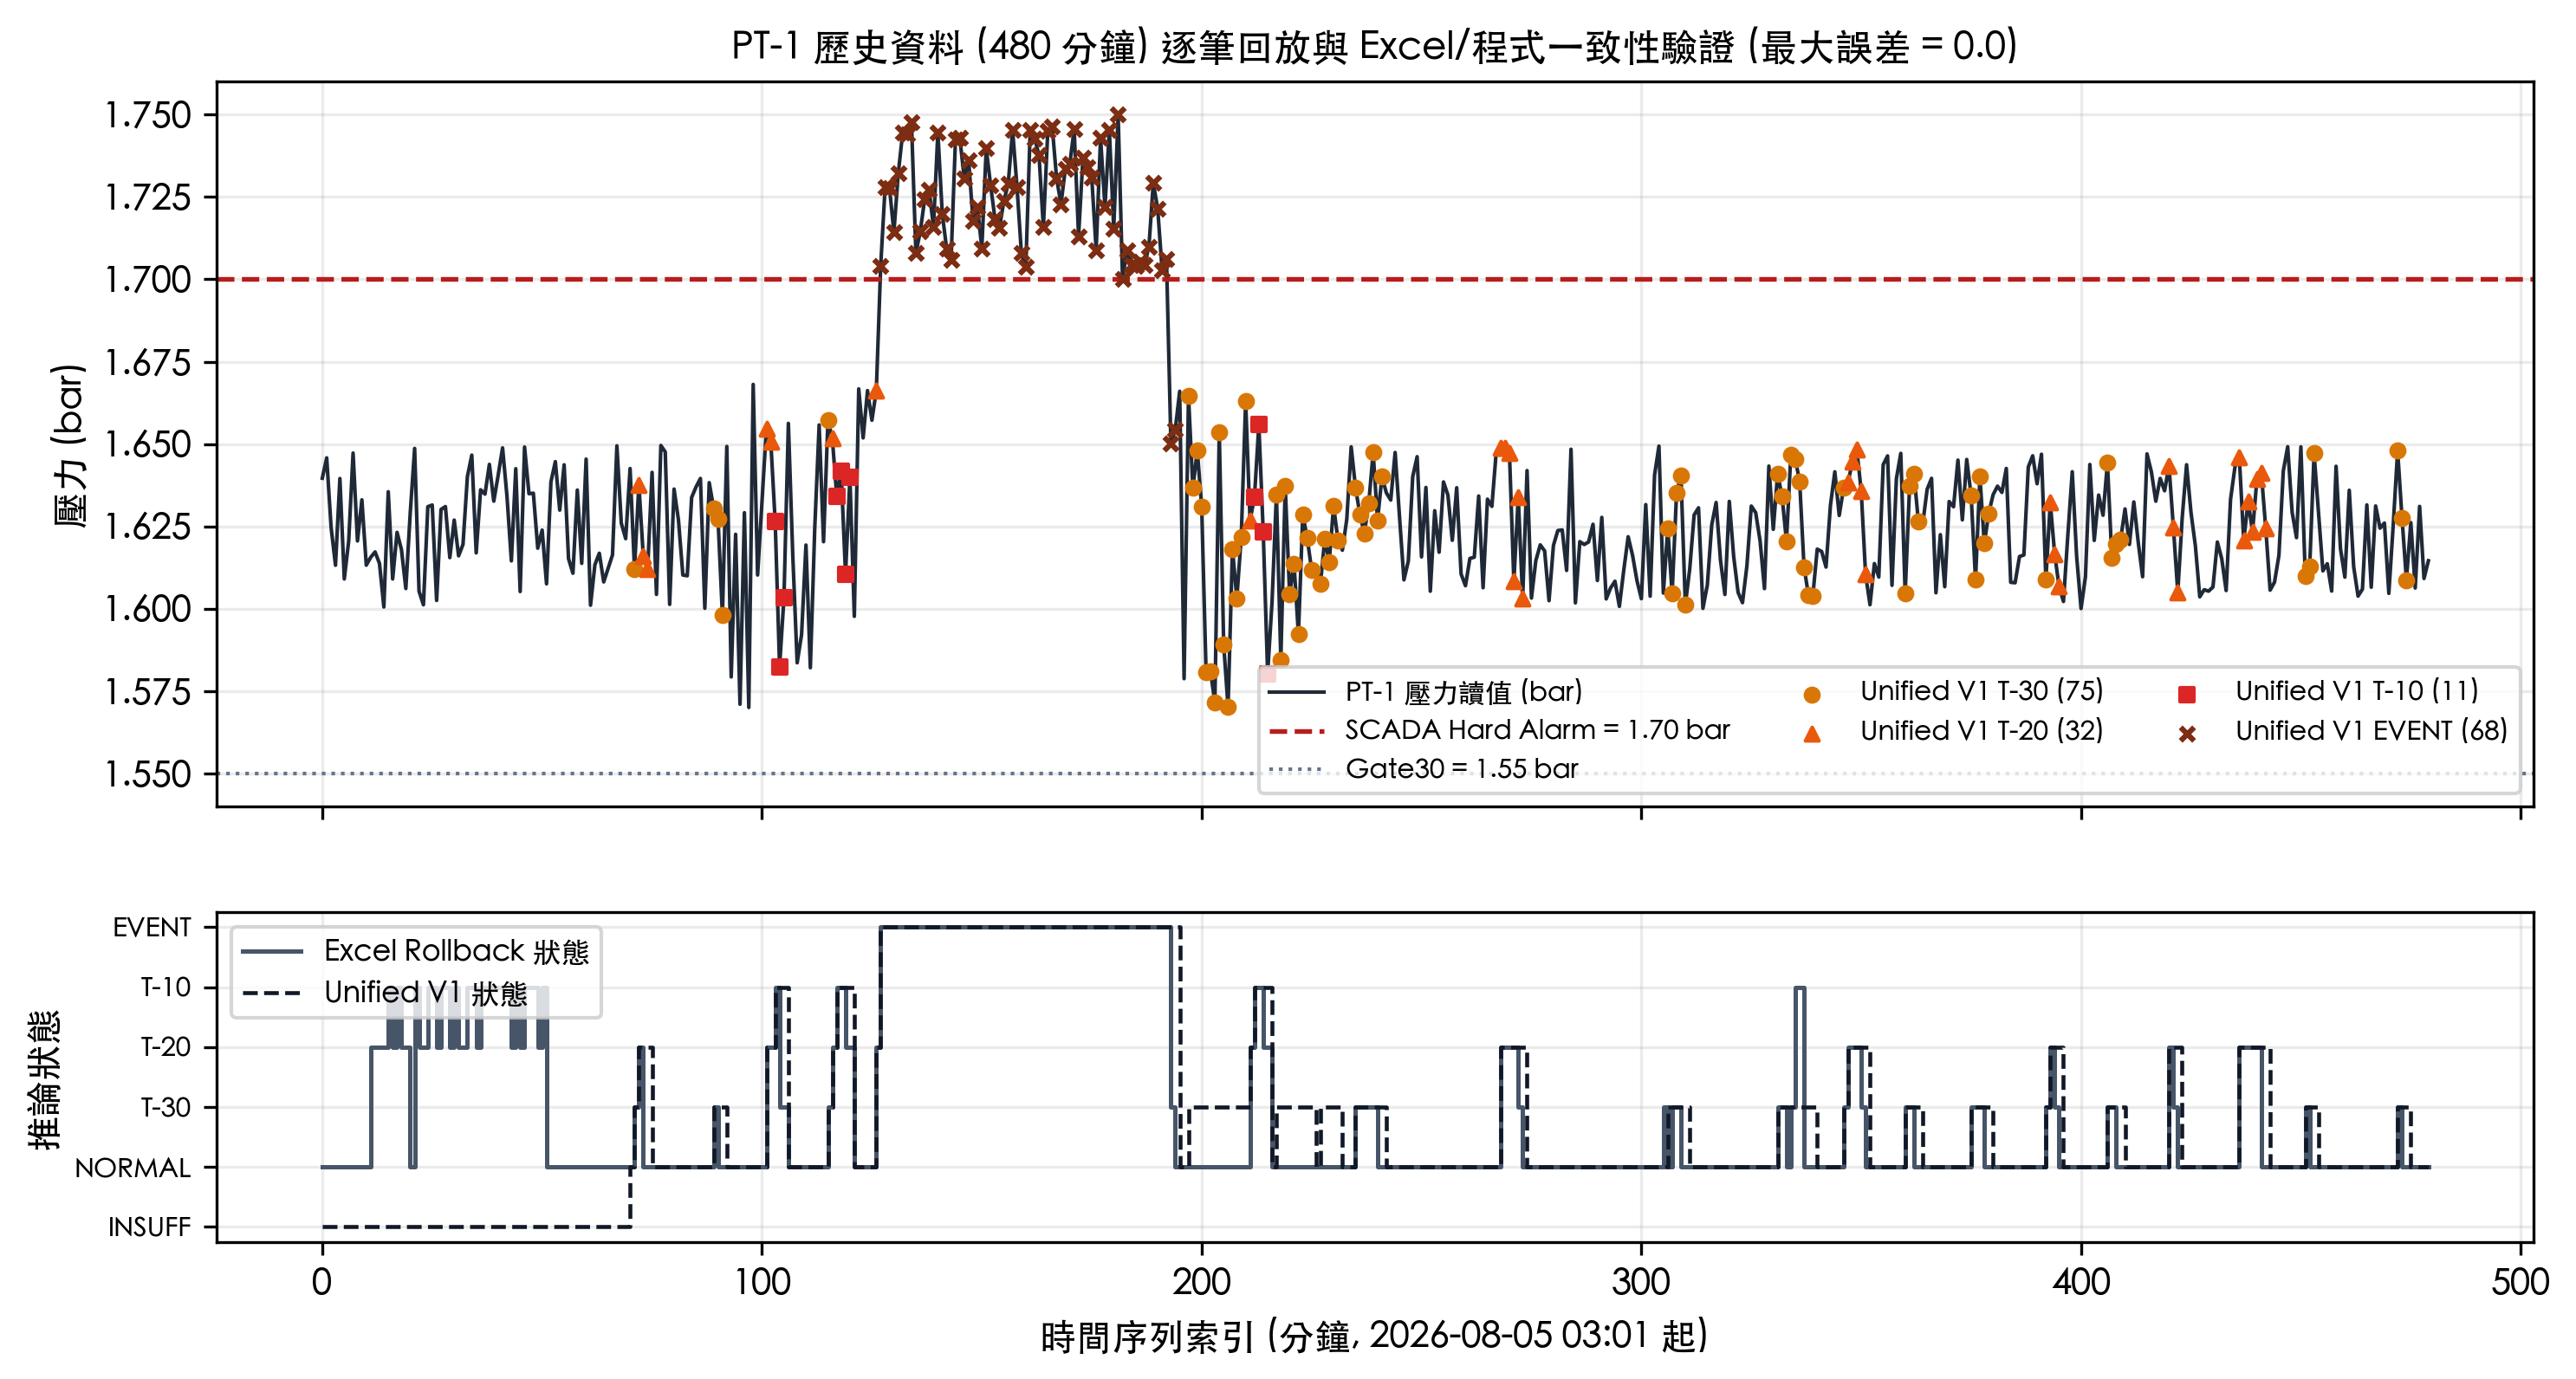
\includegraphics[width=0.95\textwidth,keepaspectratio]{picture/fig_excel_pt1_replay.png}
    \caption{Excel 參考模型 \texttt{PT-1} (480 分鐘) Past-Only 逐筆回放與狀態比較圖}
    \label{fig:excel_replay}
\end{figure}

\subsection{全廠 320 測點 (3,840 場) 公平基準比較與消融分析}
為滿足「每個感測器至少 10 次有效測試」之覆蓋率要求，本實驗針對全廠所有 \textbf{320 支感測器}（160 支 PT、80 支 FT、80 支 PDT）各設計 12 種具獨立隨機種子之受控情境：包含 8 種終將越過工程門檻之異常（慢/中/快雙向斜坡漂移各 3 種、正負階躍各 1 種）與 4 種不越限干擾或異常品質情境（常態雜訊、單分鐘 $\pm 30\%$ 跨度突波 \texttt{TRANSIENT\_SPIKE}、週期 4 分鐘震盪與連續 16 分鐘品質失效／凍結）。四種方法讀取完全相同之輸入序列與一致觸發判定。

表~\ref{tab:baseline_comp_v2} 與圖~\ref{fig:comp_1920} 呈現 160 PT 子集（1,920 場）與全廠 320 測點（3,840 場）之完整評測結果。於預設單點即刻觸發（$\text{raw\_onset}=1$）條件下，所提方法在 160 PT 子集取得 TP=1,280、TN=478、FP=162、FN=0（召回率 \textbf{100.0\%} [95\% Wilson CI: 99.70\%--100.00\%]、精確率 \textbf{88.77\%} [87.03\%--90.29\%]、F1=\textbf{0.9405}、平均提前量 \textbf{10.58 分鐘}）；與 Naive OLS（F1=0.9412、FAR=25.00\%）表現相近，尚未呈現全面超越。

\begin{table}[H]
\centering
\caption{四種異常偵測與預警方法於 160 PT (1,920 場) 與全廠 320 測點 (3,840 場) 公平比較表}
\label{tab:baseline_comp_v2}
\scriptsize
\renewcommand{\arraystretch}{1.18}
\setlength{\tabcolsep}{3pt}
\begin{tabularx}{\textwidth}{lXcccccc}
\toprule
\textbf{評估範圍} & \textbf{模型方法} & \textbf{TP/FP} & \textbf{TN/FN} & \textbf{Recall} & \textbf{Prec.} & \textbf{F1} & \textbf{FAR / Lead} \\
\midrule
160 PT & Static (ISA-18.2) & 1280 / 0   & 640 / 0 & 100.0\% & 100.0\% & 1.0000 & 0.00\% / 0.00m \\
(1,920 場) & EWMA ($\lambda=0.2, 3\sigma$) & 1280 / 349 & 291 / 0 & 100.0\% & 78.58\% & 0.8800 & 54.53\% / 12.92m \\
& Naive OLS ($k=10$) & 1280 / 160 & 480 / 0 & 100.0\% & 88.89\% & 0.9412 & 25.00\% / 10.66m \\
& \textbf{Proposed Unified V1} & 1280 / 162 & 478 / 0 & 100.0\% & 88.77\% & 0.9405 & 25.31\% / 10.58m \\
\midrule
全廠 320 測點 & Static (ISA-18.2) & 2560 / 0   & 1280 / 0 & 100.0\% & 100.0\% & 1.0000 & 0.00\% / 0.00m \\
(3,840 場) & EWMA ($\lambda=0.2, 3\sigma$) & 2560 / 687 & 593 / 0 & 100.0\% & 78.84\% & 0.8817 & 53.67\% / 12.94m \\
& Naive OLS ($k=10$) & 2560 / 321 & 959 / 0 & 100.0\% & 88.86\% & 0.9410 & 25.08\% / 10.67m \\
& \textbf{Proposed Unified V1} & 2560 / 326 & 954 / 0 & 100.0\% & 88.70\% & 0.9401 & 25.47\% / 10.59m \\
\bottomrule
\end{tabularx}
\end{table}

\begin{figure}[H]
    \centering
    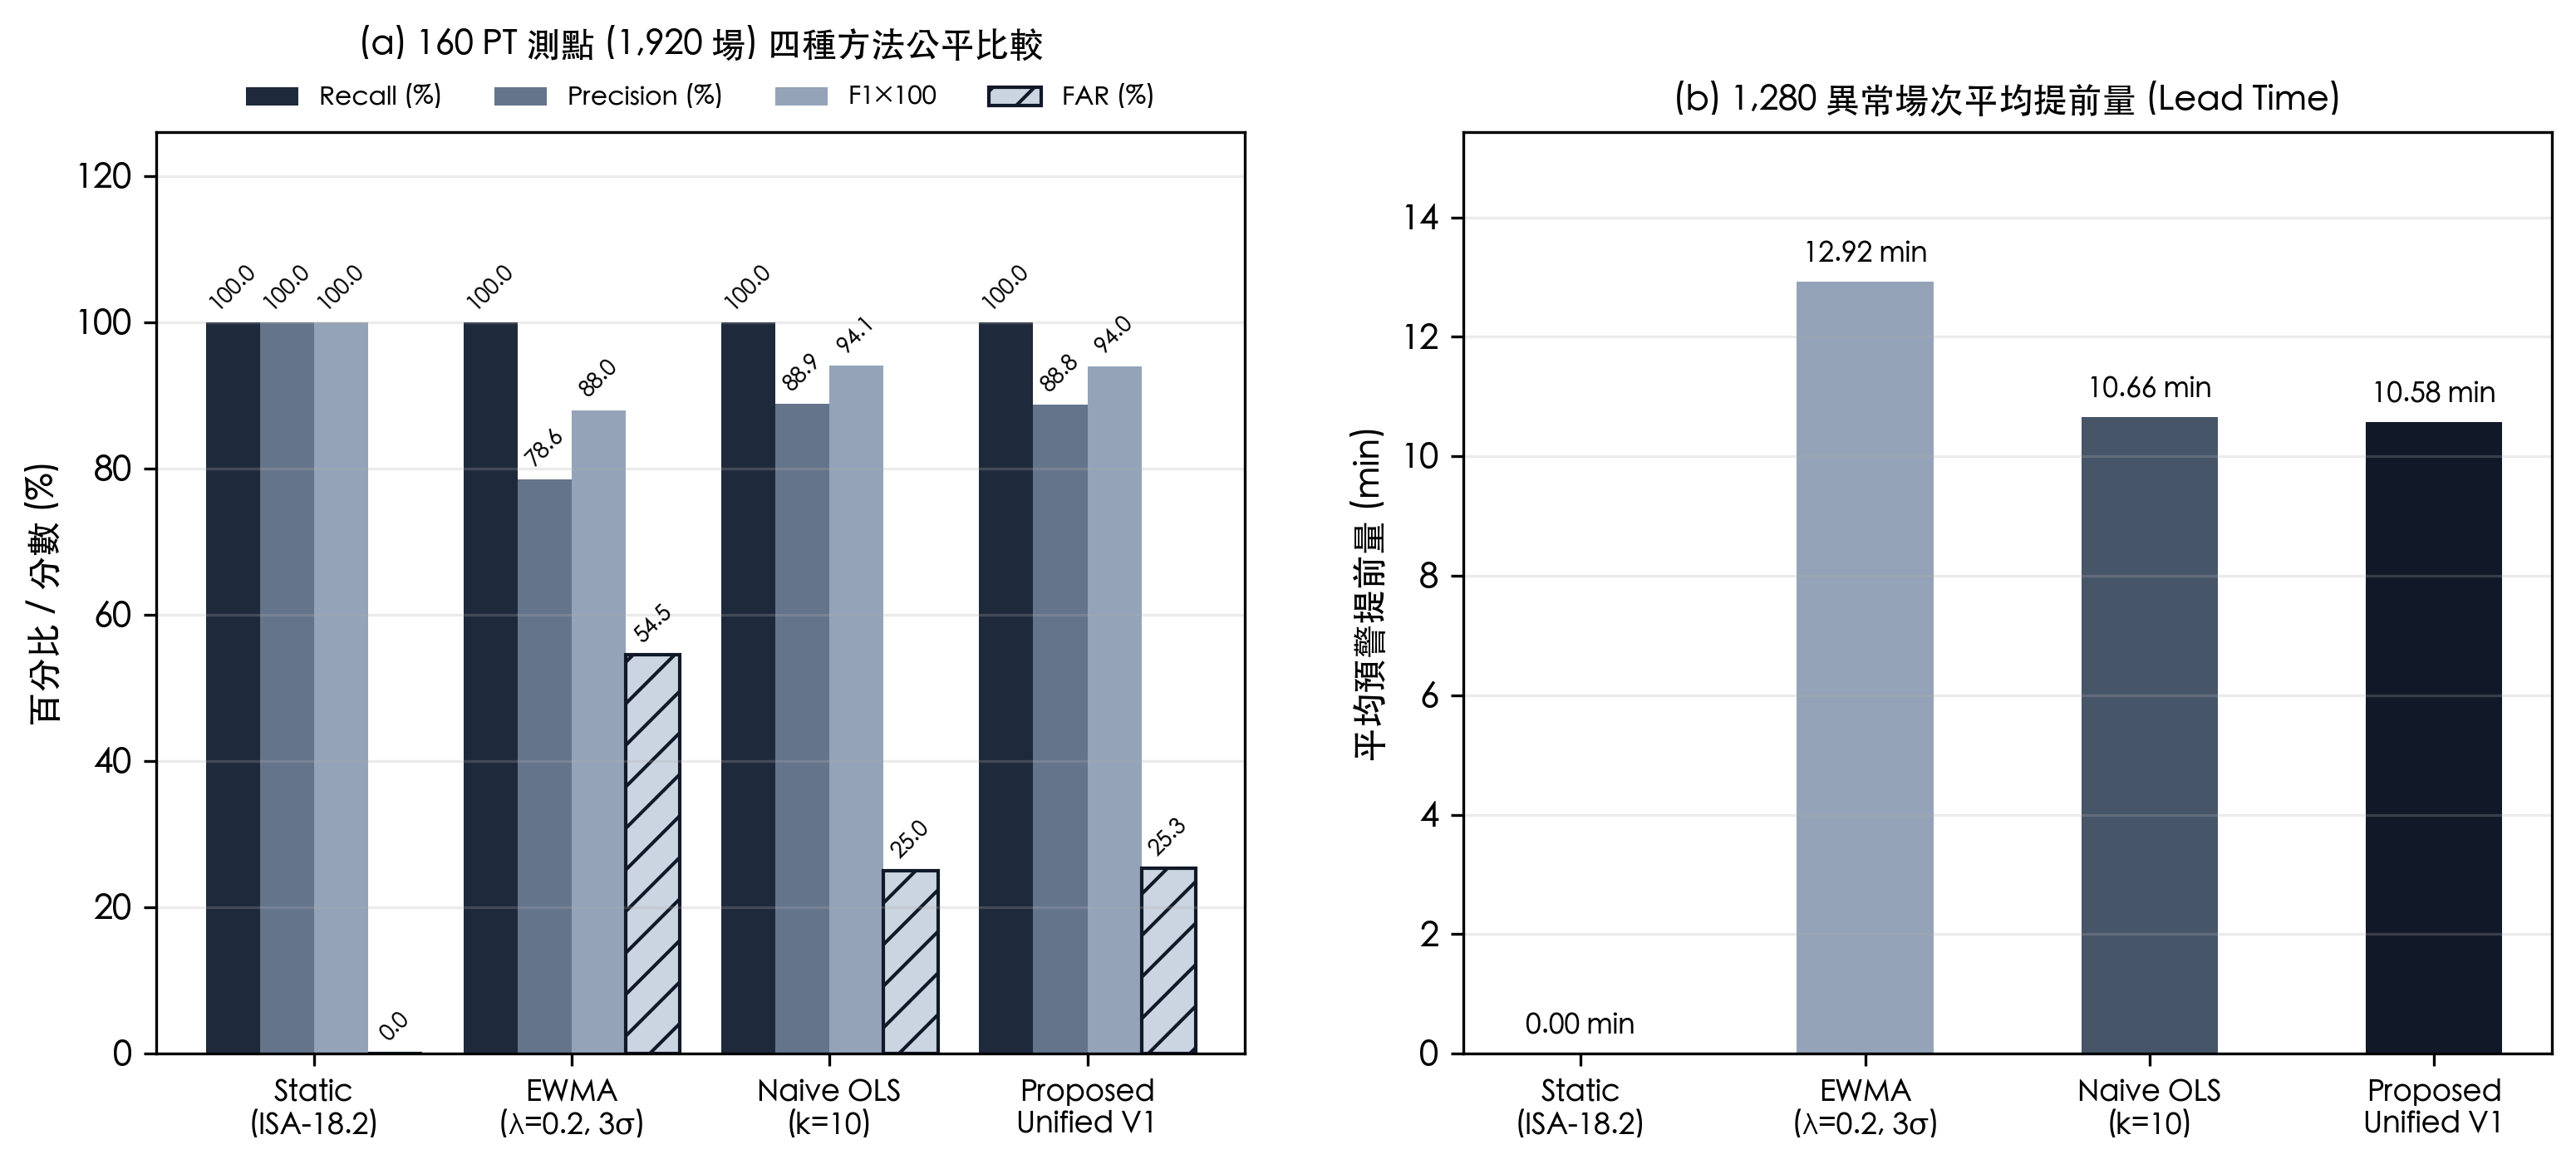
\includegraphics[width=0.95\textwidth,keepaspectratio]{picture/fig_model_comparison_1920.png}
    \caption{160 PT 測點 (1,920 場) 四種方法評估指標與平均提前量比較圖}
    \label{fig:comp_1920}
\end{figure}

針對上述 326 筆誤報進行逐筆失敗根因解剖，發現 \textbf{320 筆（98.2\%）皆發生於單分鐘 $\pm 30\%$ 跨度突波（\texttt{TRANSIENT\_SPIKE}）}。原因在於外推公式 $\hat{x}(t+30) = x_{\mathrm{now}} + \hat{\beta}\cdot 30$ 直接採用瞬時讀值作為錨點，當單點尖峰疊加局部正斜率時即刻越限，且 L6 遲滯鎖存隨即鎖定 3 分鐘。為驗證改進方案，本研究進一步於 40 PT $\times$ 12 = 480 場驗證集執行參數敏感度與前置確認消融實驗（圖~\ref{fig:ablation}）：若於進入 L6 鎖存前要求連續 2 分鐘原始預警成立（$\text{raw\_onset}=2$），於 $\theta=2.0, g=5\%$ 時誤報率可由 \textbf{25.62\% 降至 6.88\%}（F1 提升至 \textbf{0.9831}、平均提前量 9.87 分鐘）；若設定 $\theta=2.5, g=5\%$，誤報率更降至 \textbf{1.25\%}（Precision \textbf{99.38\%}、F1=\textbf{0.9969}、平均提前量 9.84 分鐘），明確證實突波誤報可透過前置防抖確認有效抑制。

\begin{figure}[H]
    \centering
    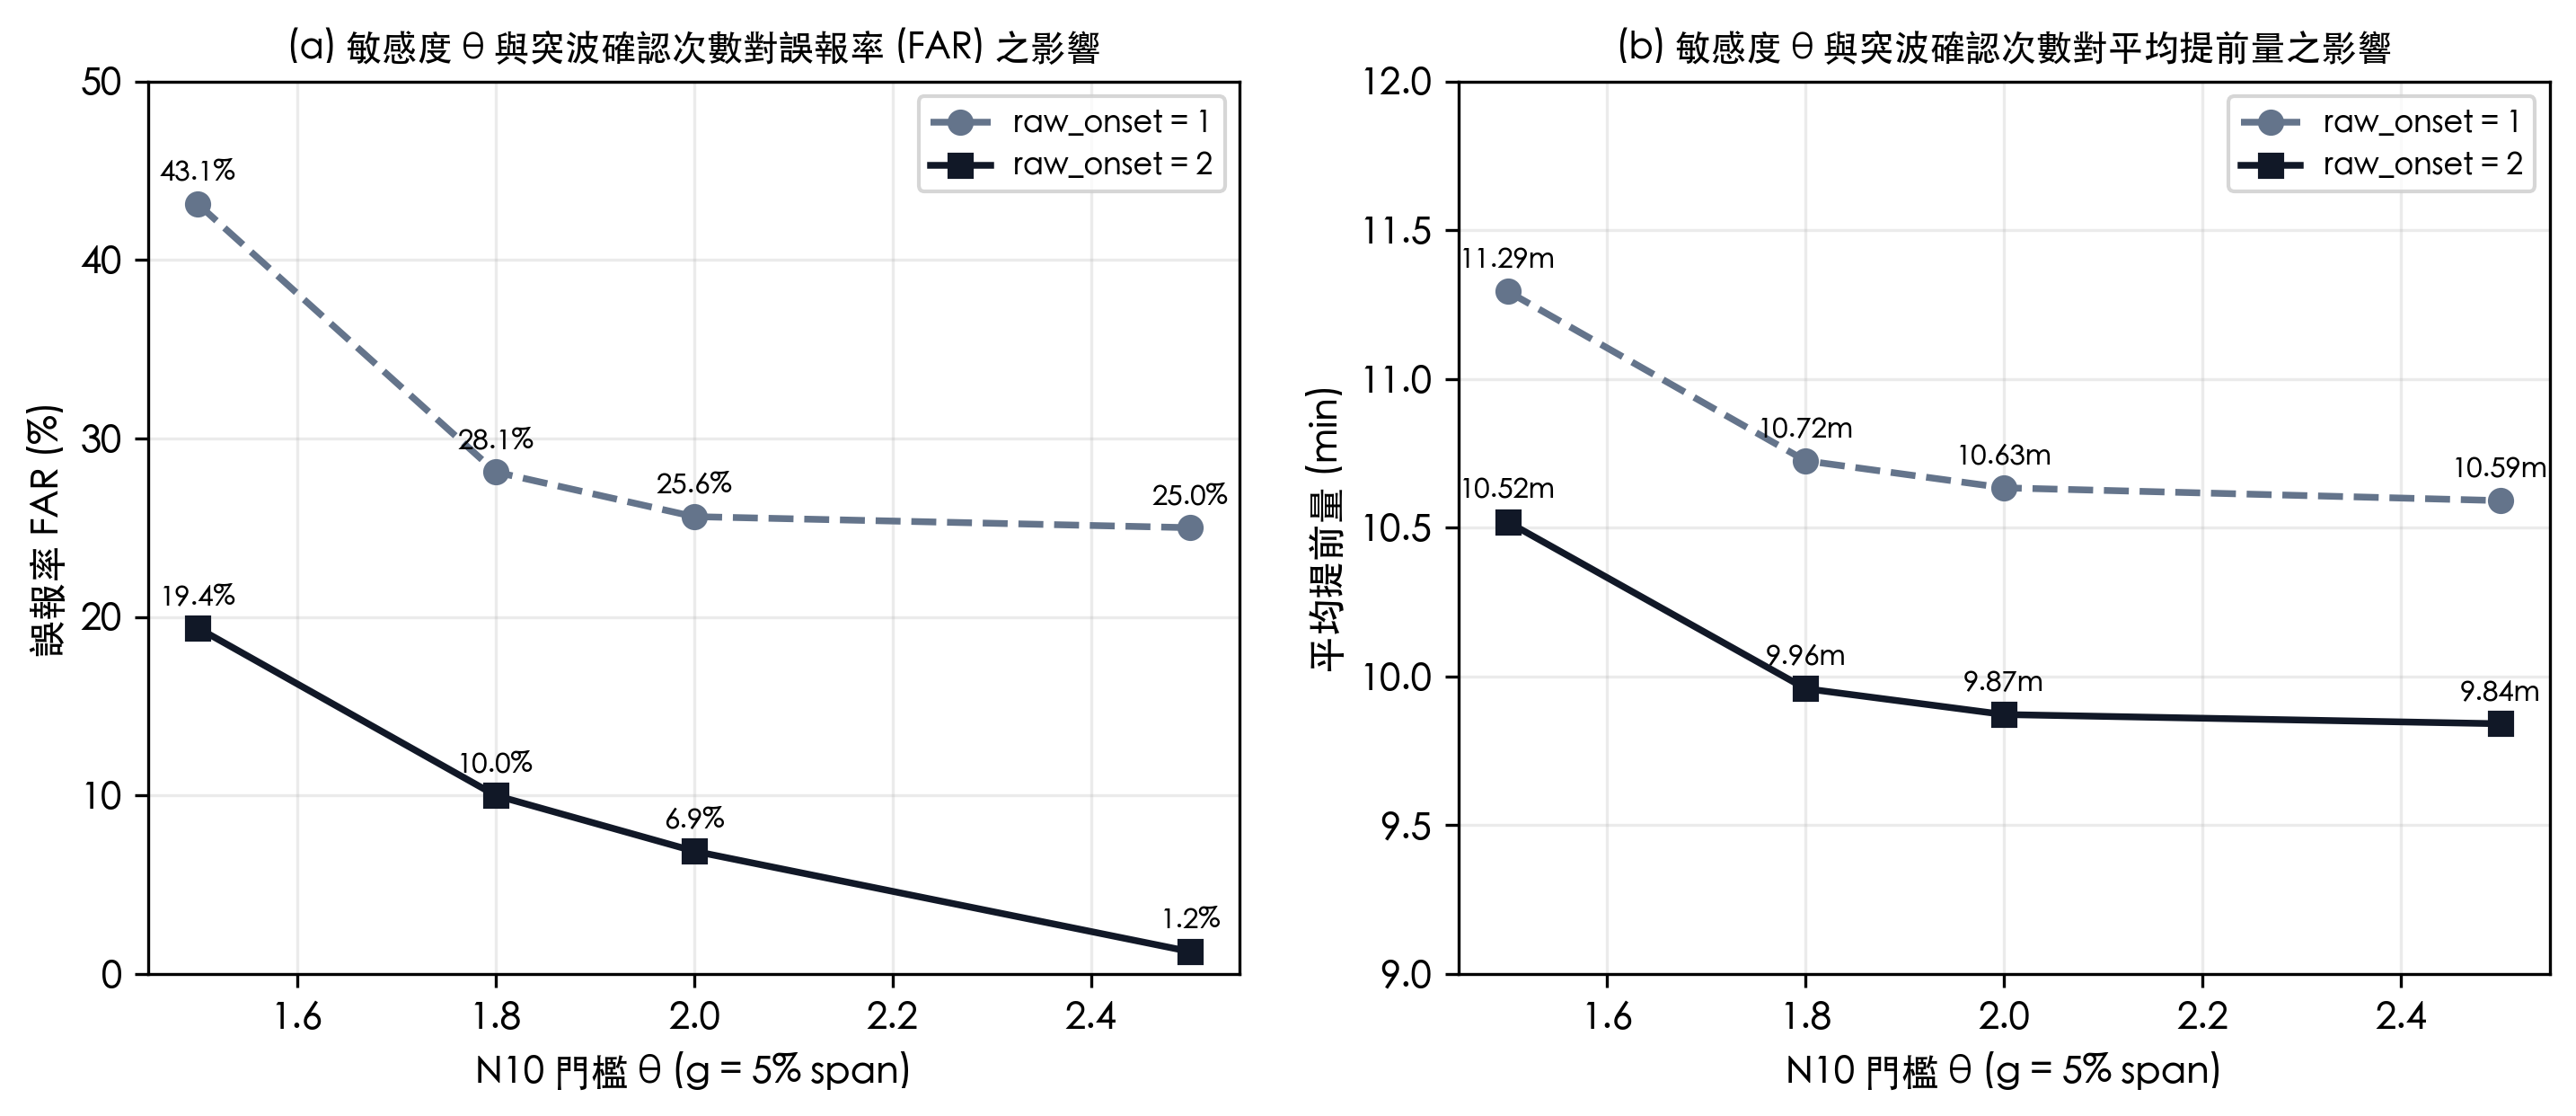
\includegraphics[width=0.95\textwidth,keepaspectratio]{picture/fig_ablation_onset_sensitivity.png}
    \caption{異常密度門檻 $\theta$ 與前置連續確認條件 ($\text{raw\_onset}=1$ vs $2$) 之誤報率與提前量消融分析}
    \label{fig:ablation}
\end{figure}

\subsection{實機推論延遲與全鏈路效能評測}
圖~\ref{fig:latency} 顯示 Apple M5 實測各層級運算耗時：單點 \texttt{evaluate\_window} 10,000 次呼叫平均 \textbf{$14.53\ \mu\mathrm{s}$}（中位數 $13.75\ \mu\mathrm{s}$、P99 $31.79\ \mu\mathrm{s}$、吞吐量 68,352 ops/s）；全廠 320 測點批次純推論（500 批）平均 \textbf{$4.68\ \mathrm{ms}$}（P99 $5.44\ \mathrm{ms}$）；全廠 320 測點推論並完整寫入 SQLite \texttt{prediction\_logs} 紀錄表（100 批）平均 \textbf{$20.54\ \mathrm{ms}$}（P99 $44.69\ \mathrm{ms}$）；真實 Modbus/TCP \texttt{FC03} 讀取 20 暫存器平均 \textbf{$271.4\ \mu\mathrm{s}$}（P99 $380.6\ \mu\mathrm{s}$）。全鏈路延遲遠低於每分鐘一次（$60,000\ \mathrm{ms}$）與每秒採樣（$1,000\ \mathrm{ms}$）之工業週期需求。

\begin{figure}[H]
    \centering
    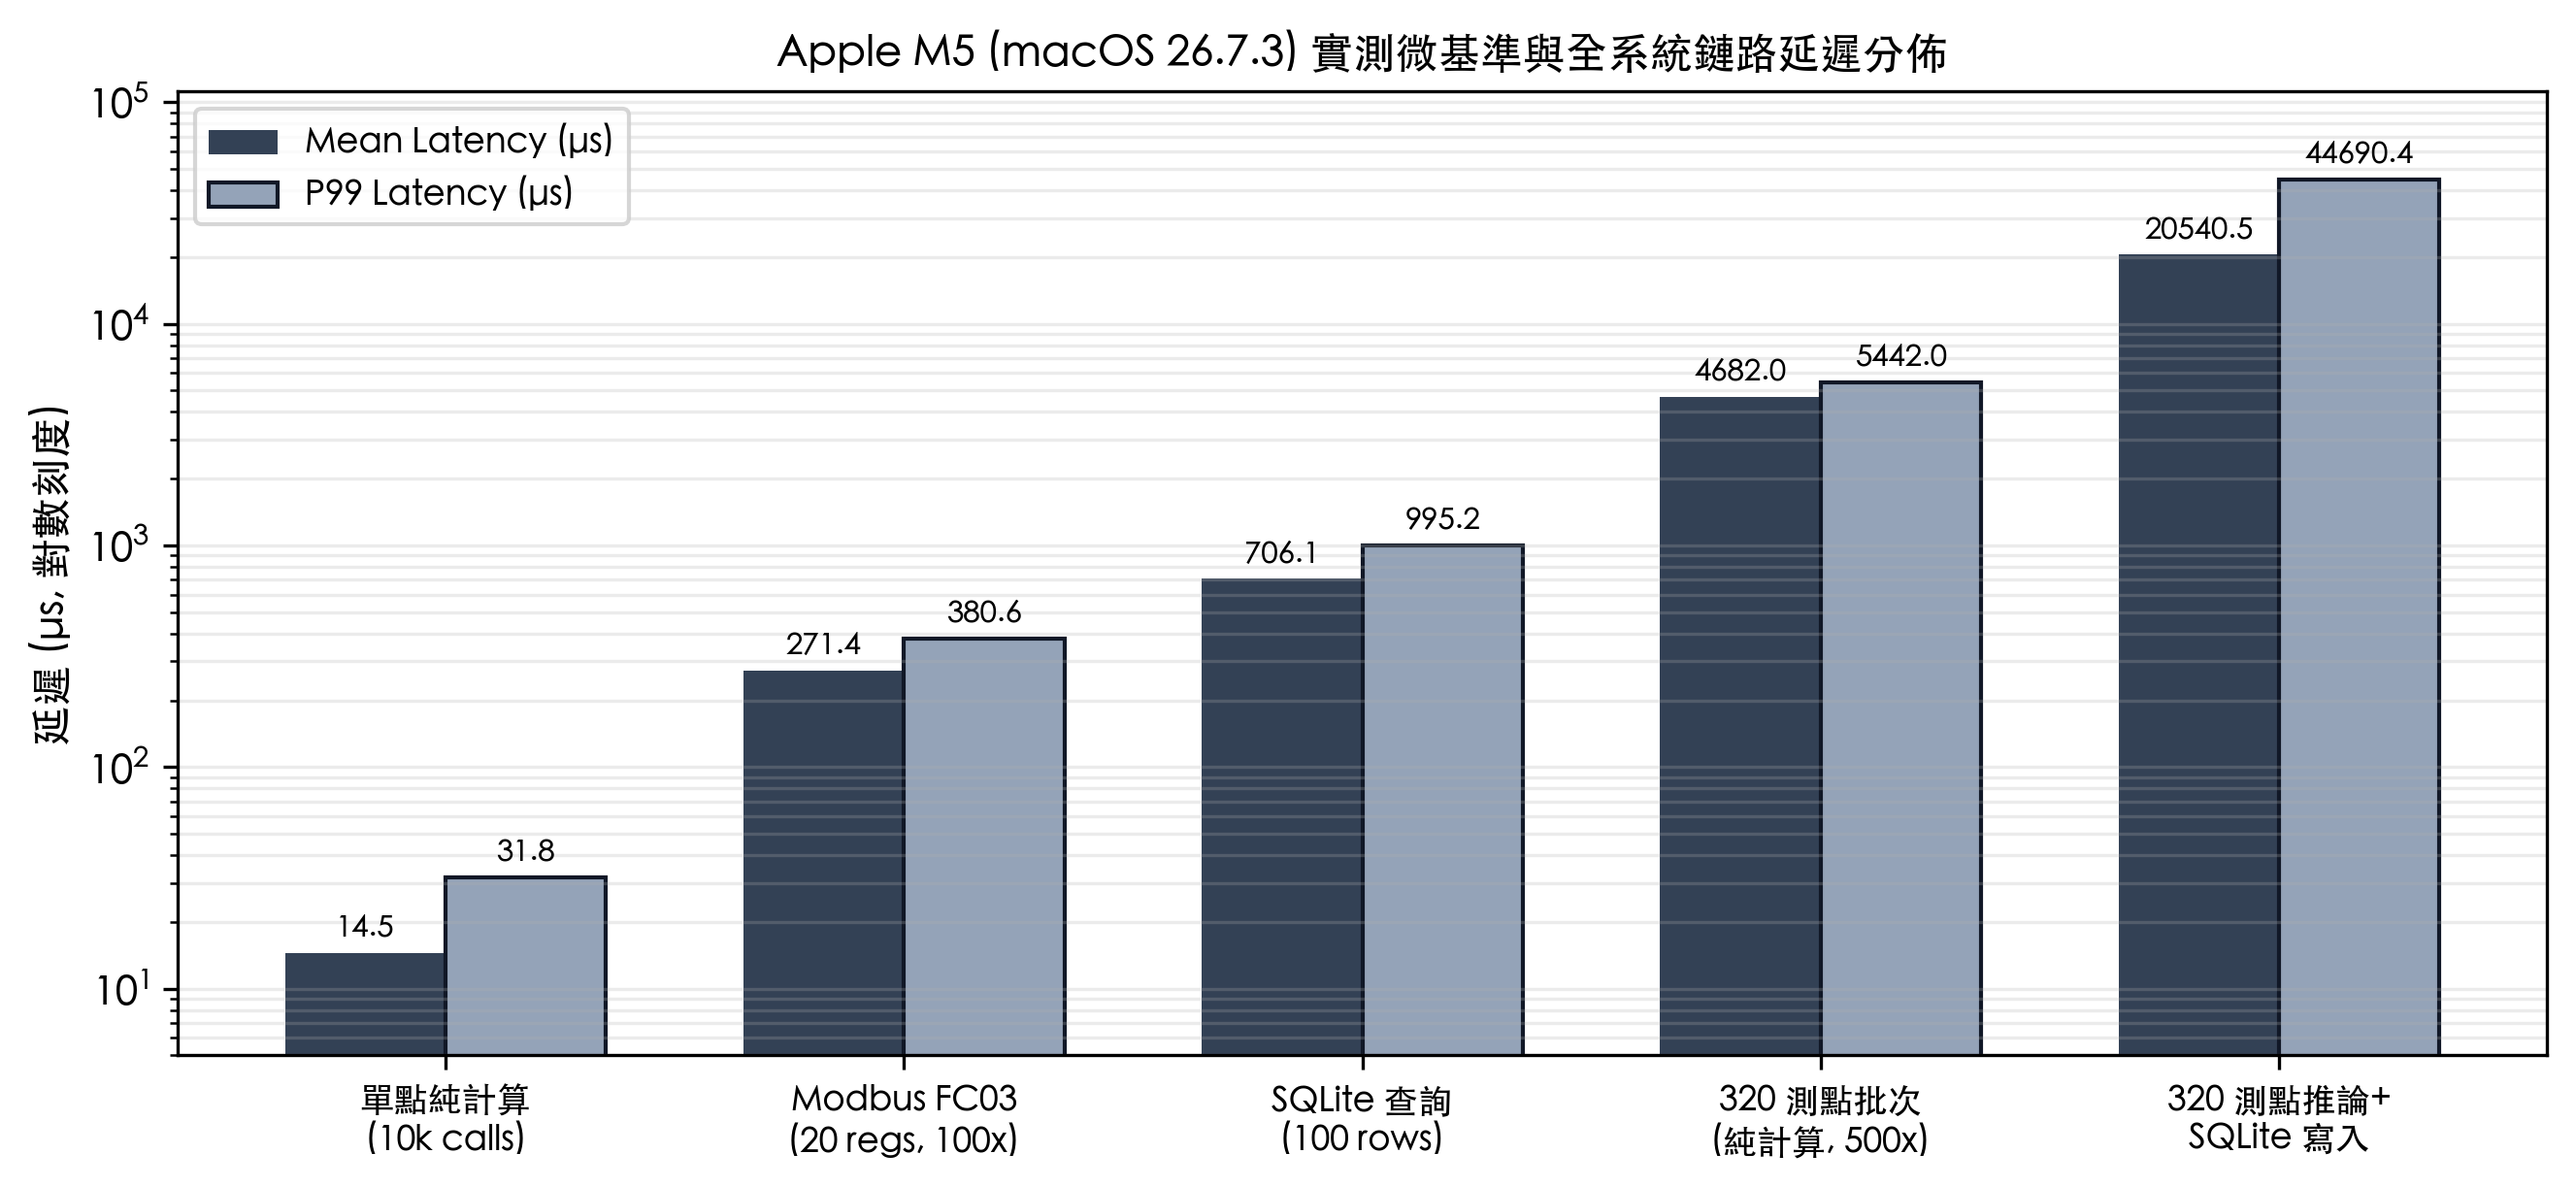
\includegraphics[width=0.92\textwidth,keepaspectratio]{picture/fig_performance_latency.png}
    \caption{Apple M5 實測單點推論、Modbus/TCP、SQLite 與 320 測點批次延遲分佈圖}
    \label{fig:latency}
\end{figure}

\subsection{線上部署系統與本機重構系統實時 11.35 分鐘驗證與截圖比較}
為驗證系統在真實時間尺度下的行為偏差偵測能力與畫面一致性，本研究於 2026 年 11 月 11 日以無頭 Google Chrome (157.0.8103.40) 透過 Puppeteer 連線至線上部署網址（\url{https://pcw-scada-system.vercel.app/}，實測持續 \textbf{11.12 分鐘}）與最新重構 v2.0 全端系統（\url{http://127.0.0.1:8000/}，採用 SSE \texttt{/api/stream} 即時推播並搭配 Port 15020 Modbus/TCP 伺服器，實測持續 \textbf{11.35 分鐘}），巡檢全部 9 個功能頁並執行全廠所有 **320 支感測器**之基準行為偏差與預警留存測試（全程零 console/page error）。

\begin{enumerate}
    \item \textbf{狀態一致性實機對照（1.72 bar 超限測試）}：於線上舊版對 \texttt{PCW01.Submain01.PTS} 注入 1.72 bar（HI=1.70 bar）後，Alarm Center 產生 \texttt{HIGH / ACTIVE\_UNACK}，惟 System Prediction 仍顯示 \texttt{NORMAL}（圖~\ref{fig:ui_defect}）；於本機重構 v2.0 版執行相同注入後，Alarm Center 與 System Prediction 同步即時顯示 \texttt{HIGH} 與 \texttt{EVENT}（Risk=100，圖~\ref{fig:ui_consistent}），確認原缺陷已修復。
    \item \textbf{超過 10 分鐘全廠 320 測點 Modbus 基準行為偏差連續實測}：透過 Modbus 模擬器將全廠 320 支測點同步調整基準並對 \texttt{PCW01.Submain01.PTS} 與 \texttt{PCW05.Submain01.PTS} 疊加 $+0.008\ \mathrm{bar/min}$ 慢速漂移（包含 160 支 PT 供／回水偏移，\texttt{PCW01–04.FT} 由 $180\to 195\ \mathrm{L/min}$ 與 80 支 \texttt{PDT} 由 $0.30\to 0.45\ \mathrm{bar}$ 之限值內偏差，另有 \texttt{PCW05–08.FT} 由 $260/240\to 195\ \mathrm{L/min}$ 越過下限觸發工程事件）。實測軌跡如圖~\ref{fig:realtime_11min} 所示：
    \begin{itemize}
        \item 本機重構 v2.0 系統於 $t=0.52\ \mathrm{min}$ 即驅動全廠 **320 / 320 支感測器**累計全數進入預警或事件判定（280 支進入預警並產生 280 筆 \texttt{DRIFT} 警報、40 支 \texttt{PCW05–08.FT} 進入 \texttt{EVENT}）；於 $t=11.35\ \mathrm{min}$ 結束時，仍有 **81 支 PT + 59 支 FT/PDT 共 140 支**依修正後 L2 水準偏移閘門穩定維持 \texttt{T-30} 預警（另有 42 支處於 \texttt{EVENT}，Alarm Center 共計 367 筆 \texttt{DRIFT} 預警事件與 42 筆硬限界警報）。SQLite \texttt{prediction\_logs} 資料表實測完整保存 \textbf{203,840 筆}涵蓋全部 320 測點之逐點推論紀錄（其中 182,597 筆為非正常狀態紀錄）。
        \item 相對地，線上舊版於 $t=10.48\ \mathrm{min}$ 處，因 \texttt{PCW01.Submain01.PTS} 局部斜率趨近於 0 且欠缺水準偏移閘門，即使此時 $N_{10}=3.53 > 2.0$ 仍退回 \texttt{NORMAL}，直接驗證本論文第~\ref{sec:drift_detection} 節偏移偵測數學修正之必要性。
    \end{itemize}
    \item \textbf{重構系統 v2.0 全介面實機展示}：系統總覽（圖~\ref{fig:ui_overview_new}）即時呈現 \texttt{320 Tags}（\texttt{160 PT · 80 FT · 80 PDT}）與 SQLite 紀錄筆數；於 11.35 分鐘實測結束時，新增之 Pair Level（80 組 Submain 配對）診斷頁面（圖~\ref{fig:ui_pair_new}）區分 \texttt{COUPLED\_DRIFT}（22 組）與單側異常；Modbus 模擬器與行為偏差場景注入面板（圖~\ref{fig:ui_injector_new}）直接連結 Port 15020 保持暫存器；Historian 歷史趨勢頁面（圖~\ref{fig:ui_historian_new}）則完整記錄 \texttt{PCW01.Submain01.PTS} 於 11.35 分鐘內隨漂移爬升與外推預測之真實時序軌跡。
\end{enumerate}

\begin{figure}[H]
    \centering
    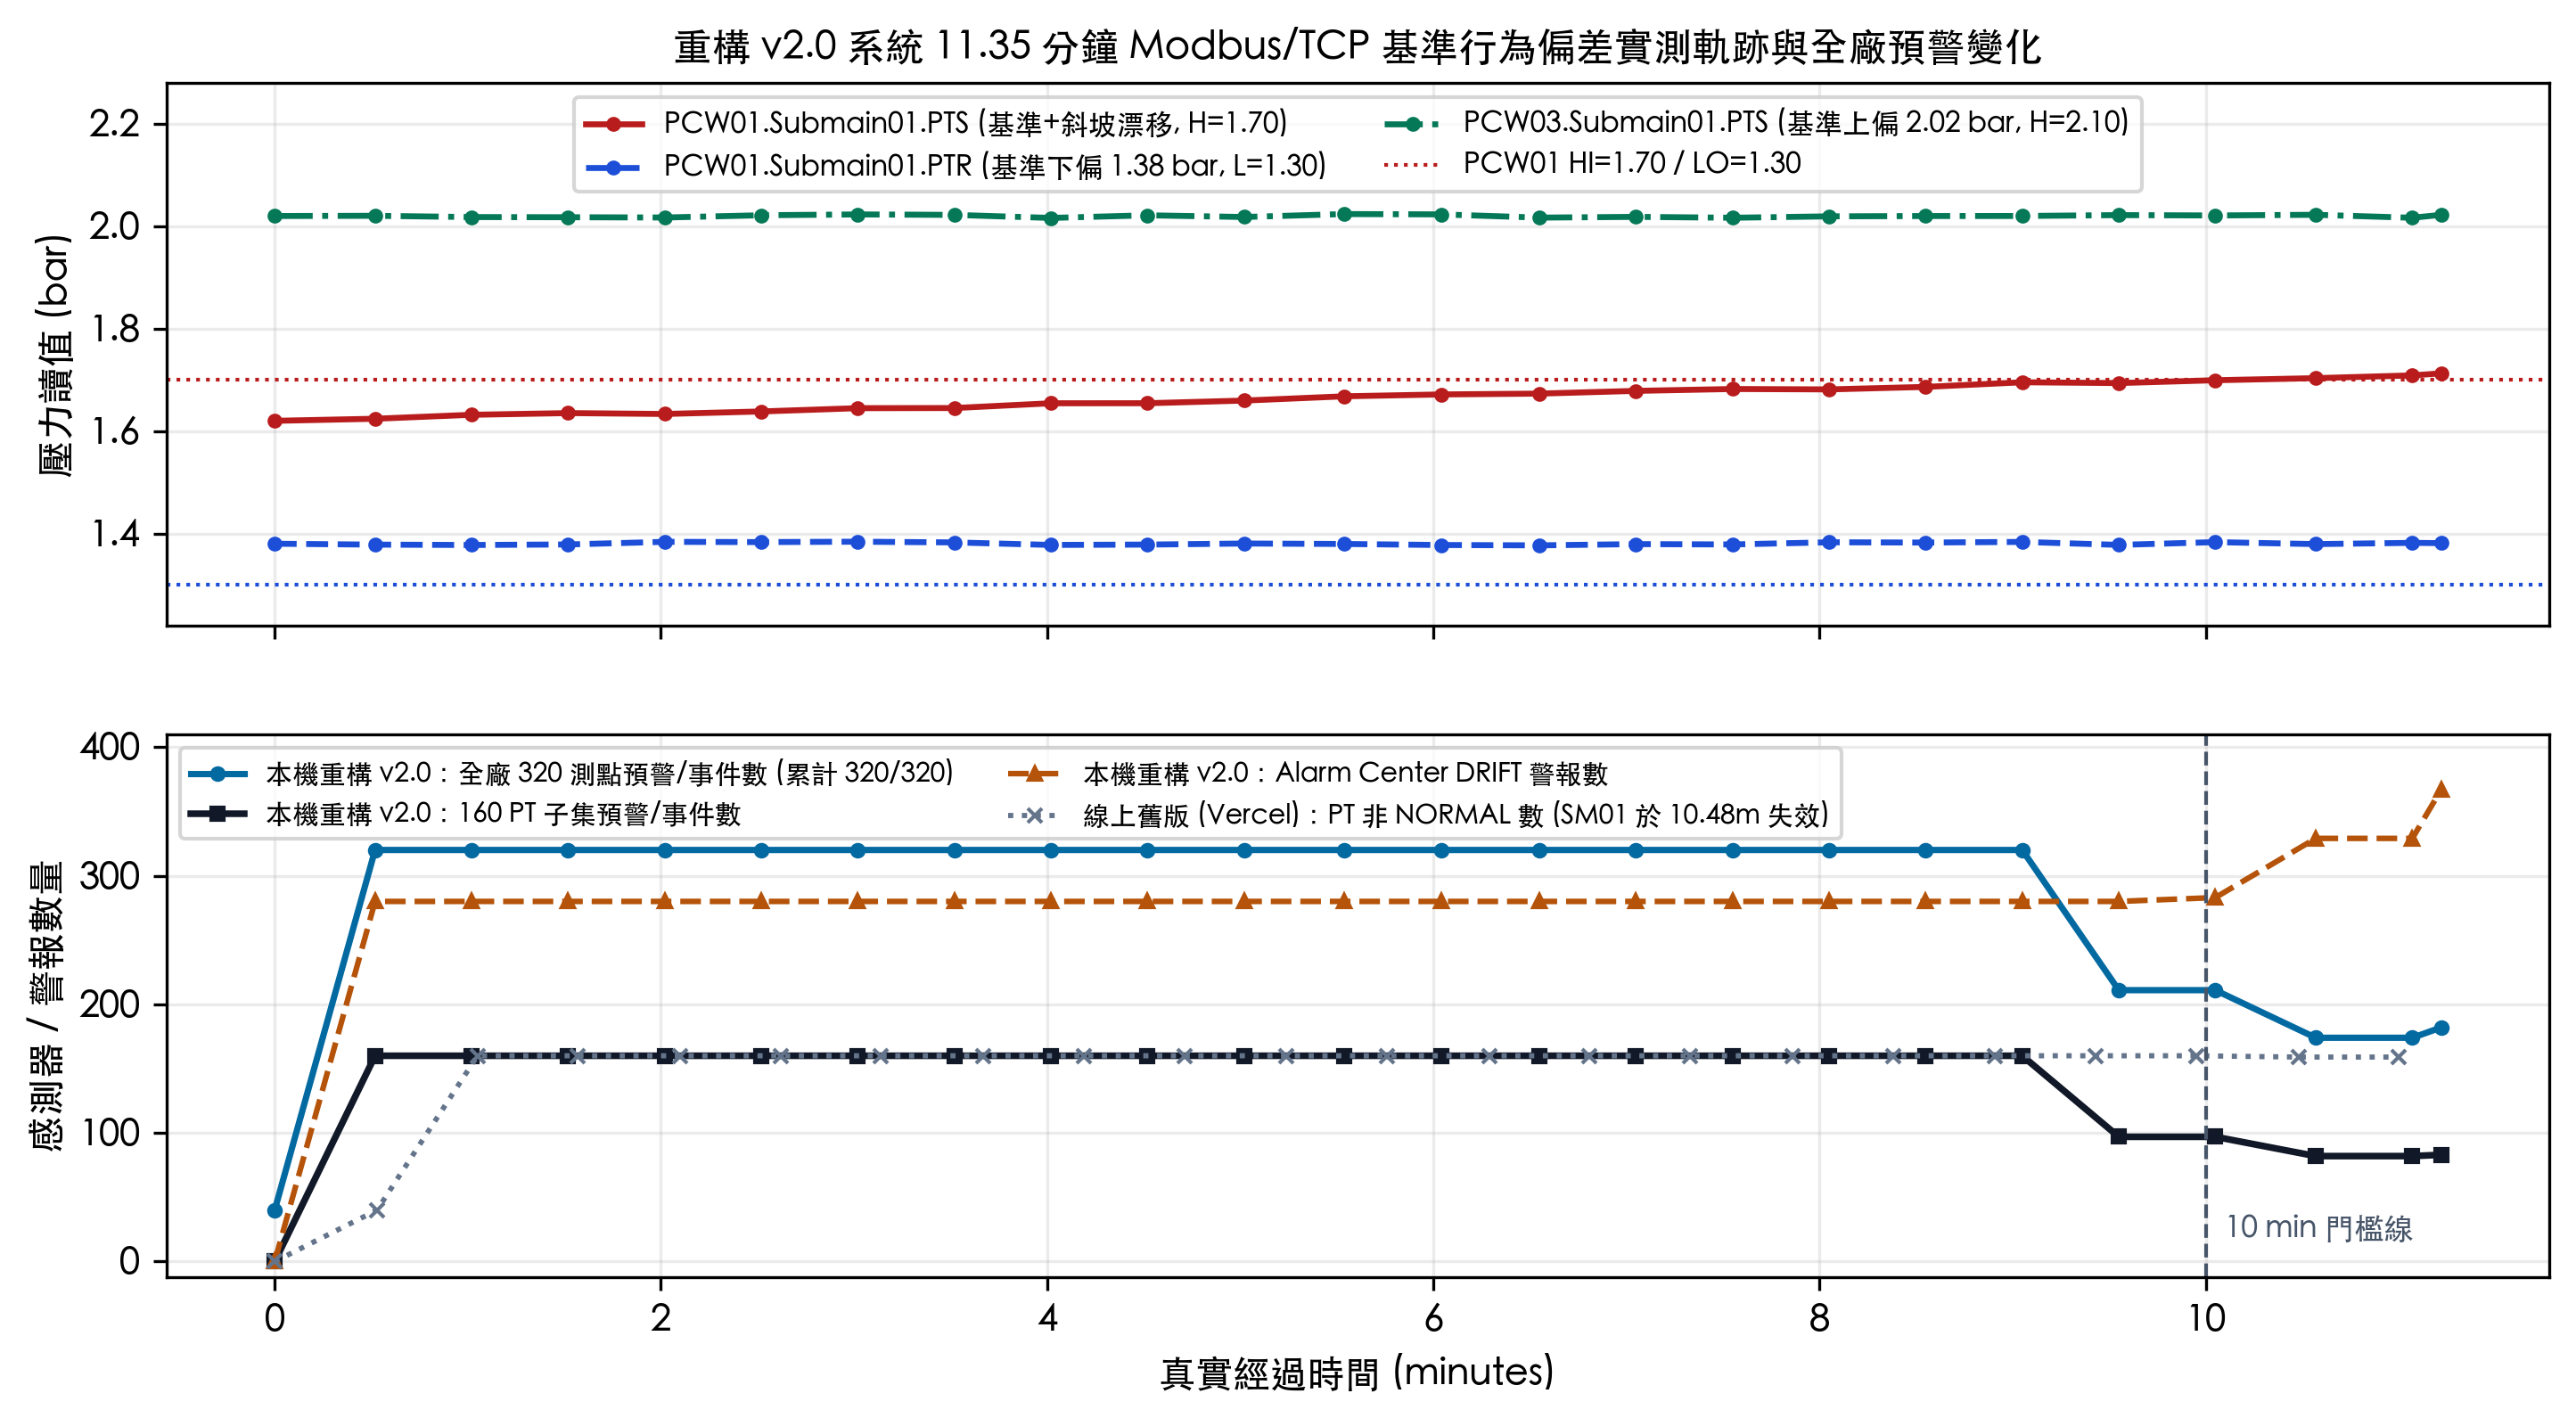
\includegraphics[width=0.95\textwidth,keepaspectratio]{picture/fig_11min_realtime_deviation.png}
    \caption{線上舊版 (11.12 分鐘) 與本機重構 v2.0 系統 (11.35 分鐘) 即時 Modbus 行為偏差實測軌跡對比圖}
    \label{fig:realtime_11min}
\end{figure}

\begin{figure}[H]
    \centering
    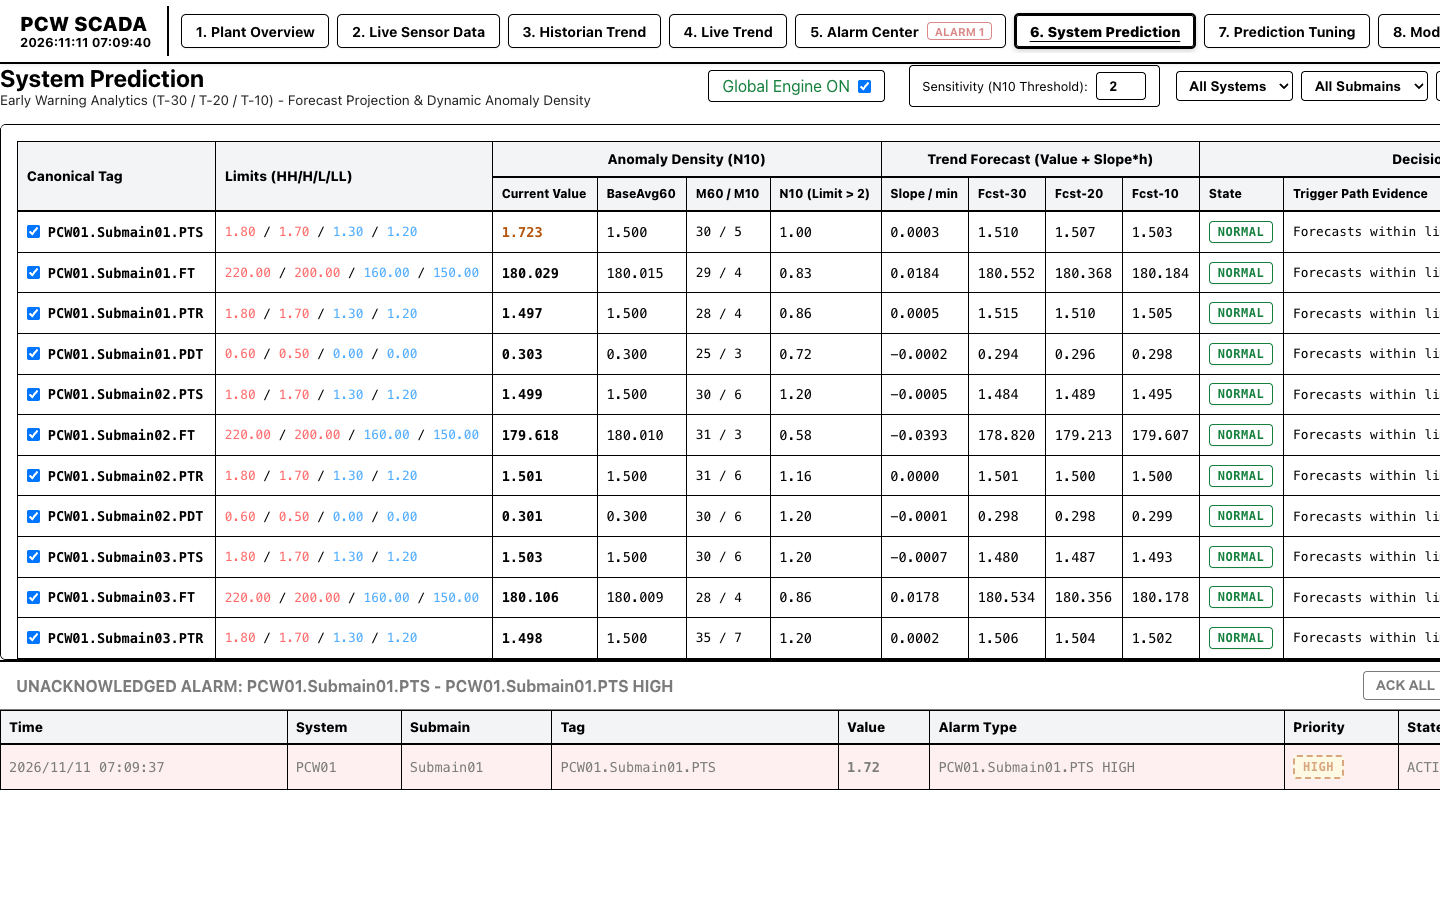
\includegraphics[width=0.92\textwidth,keepaspectratio]{picture/ui_deployed_defect.png}
    \caption{線上舊版 (\texttt{vercel.app}) 1.72 bar 超限時 Alarm Center 與 System Prediction 狀態不一致實測截圖}
    \label{fig:ui_defect}
\end{figure}

\begin{figure}[H]
    \centering
    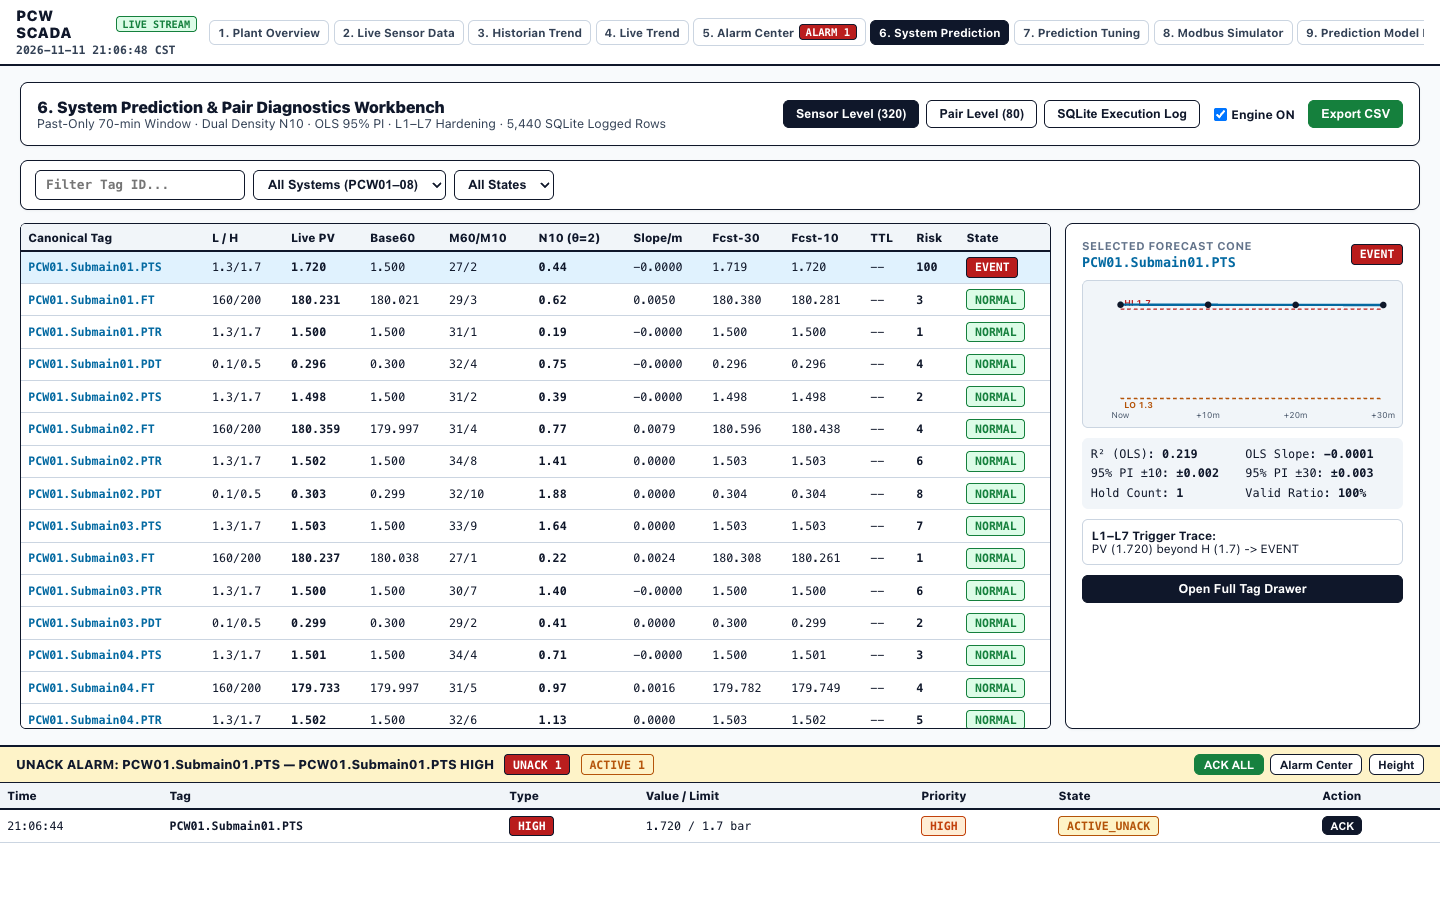
\includegraphics[width=0.92\textwidth,keepaspectratio]{picture/ui_local_consistent_pred.png}
    \caption{本機重構系統修復後 1.72 bar 超限同步呈現 \texttt{EVENT} 與 \texttt{HIGH} 警報實測截圖}
    \label{fig:ui_consistent}
\end{figure}

\begin{figure}[H]
    \centering
    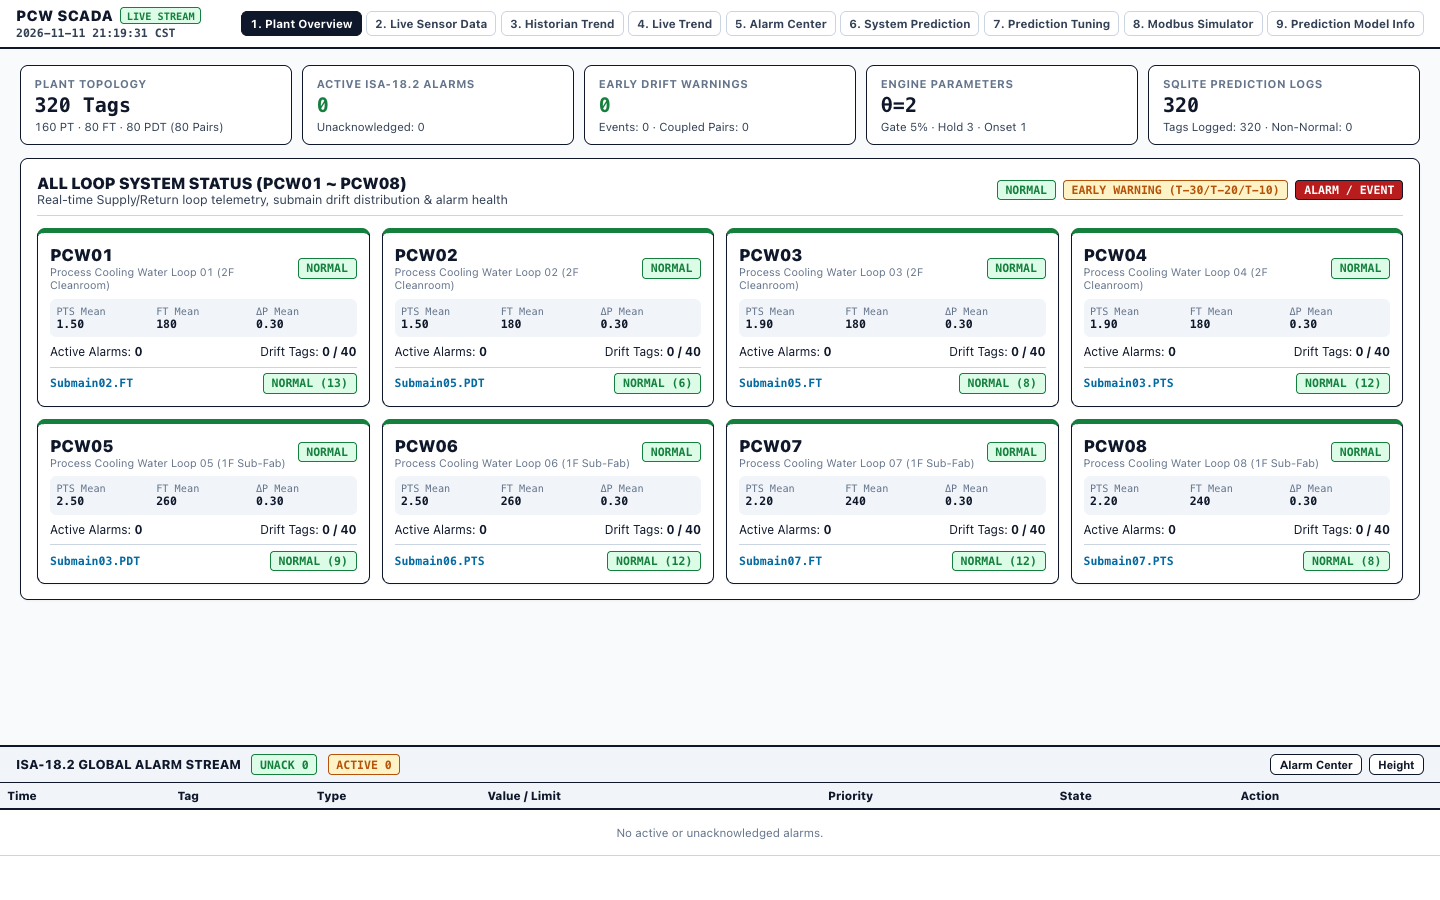
\includegraphics[width=0.92\textwidth,keepaspectratio]{picture/ui_local_overview.png}
    \caption{重構系統 v2.0 全廠八套 PCW 迴路總覽與 SQLite 統計指標最新介面}
    \label{fig:ui_overview_new}
\end{figure}

\begin{figure}[H]
    \centering
    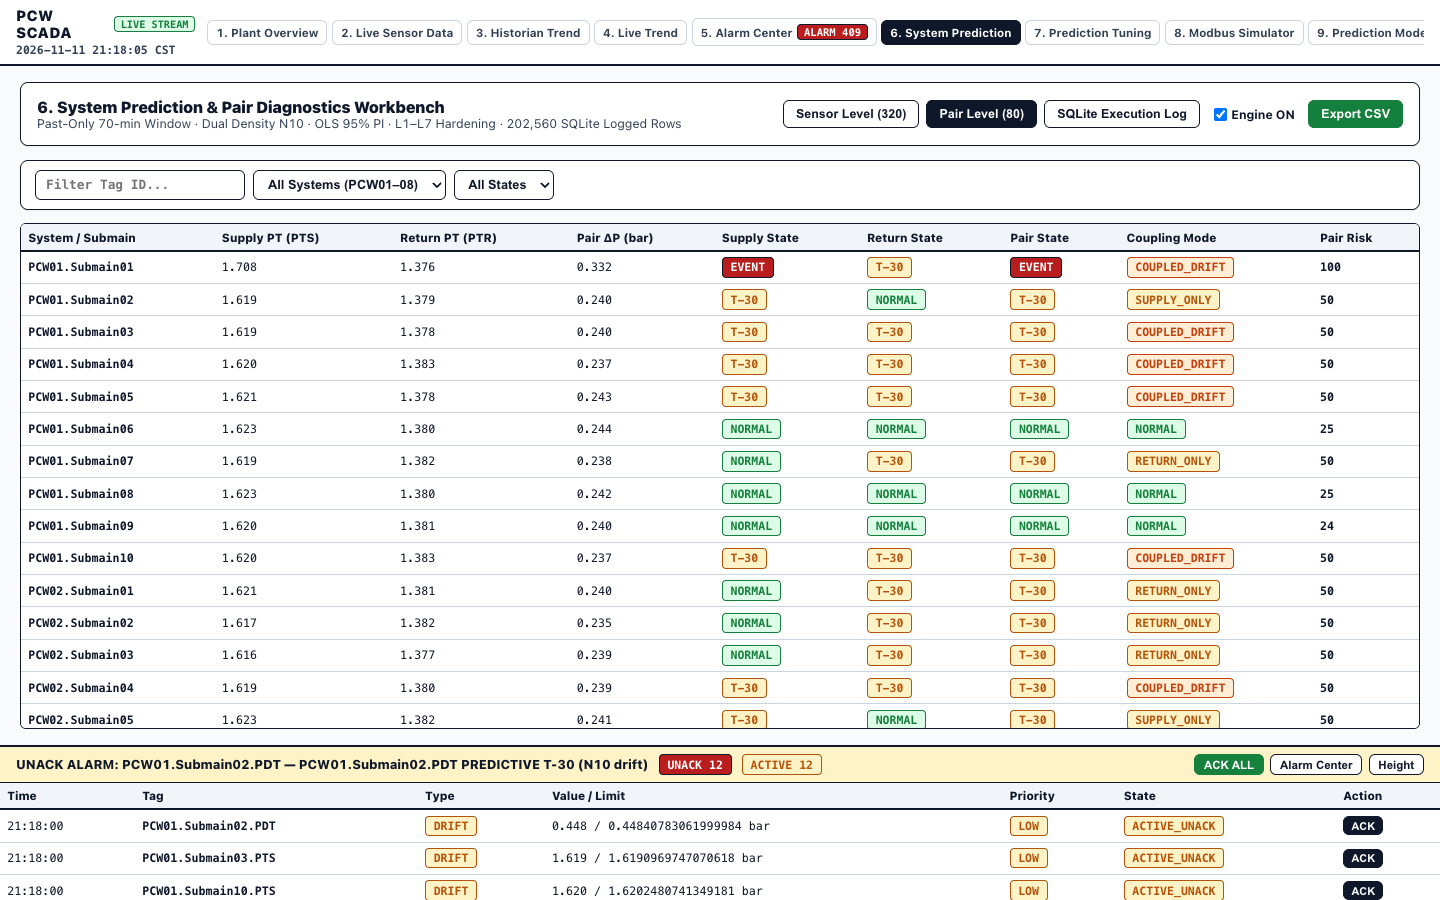
\includegraphics[width=0.92\textwidth,keepaspectratio]{picture/ui_local_pair_diag.png}
    \caption{本機重構系統新增 Submain 供回水配對層級 (Pair Level) 預警診斷畫面}
    \label{fig:ui_pair_new}
\end{figure}

\begin{figure}[H]
    \centering
    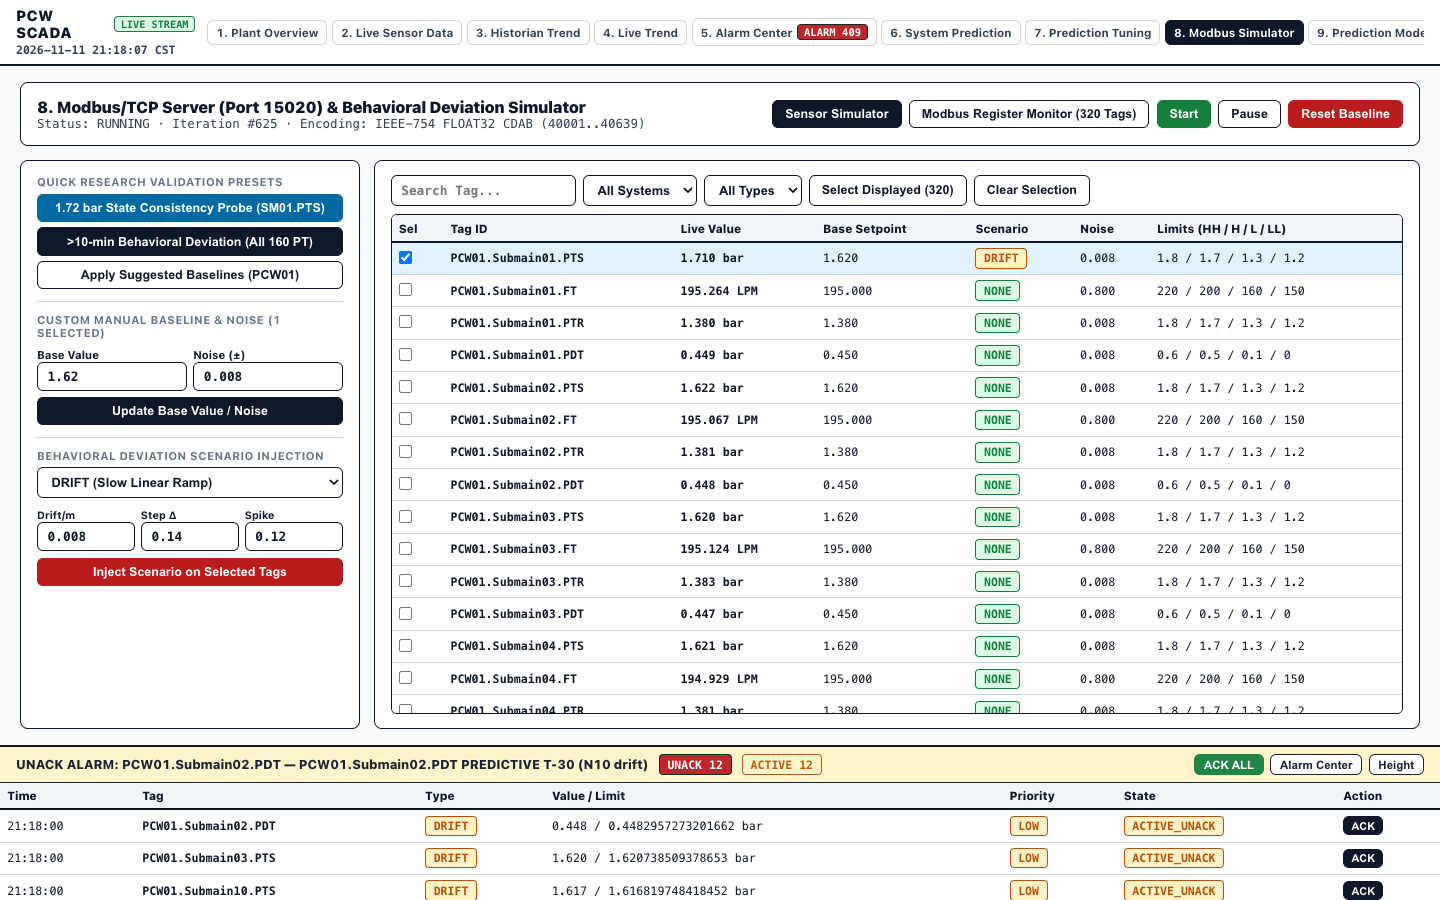
\includegraphics[width=0.92\textwidth,keepaspectratio]{picture/ui_local_fault_injector.png}
    \caption{本機重構系統 Modbus/TCP 模擬器與多種行為偏差情境注入面板實測截圖}
    \label{fig:ui_injector_new}
\end{figure}

\begin{figure}[H]
    \centering
    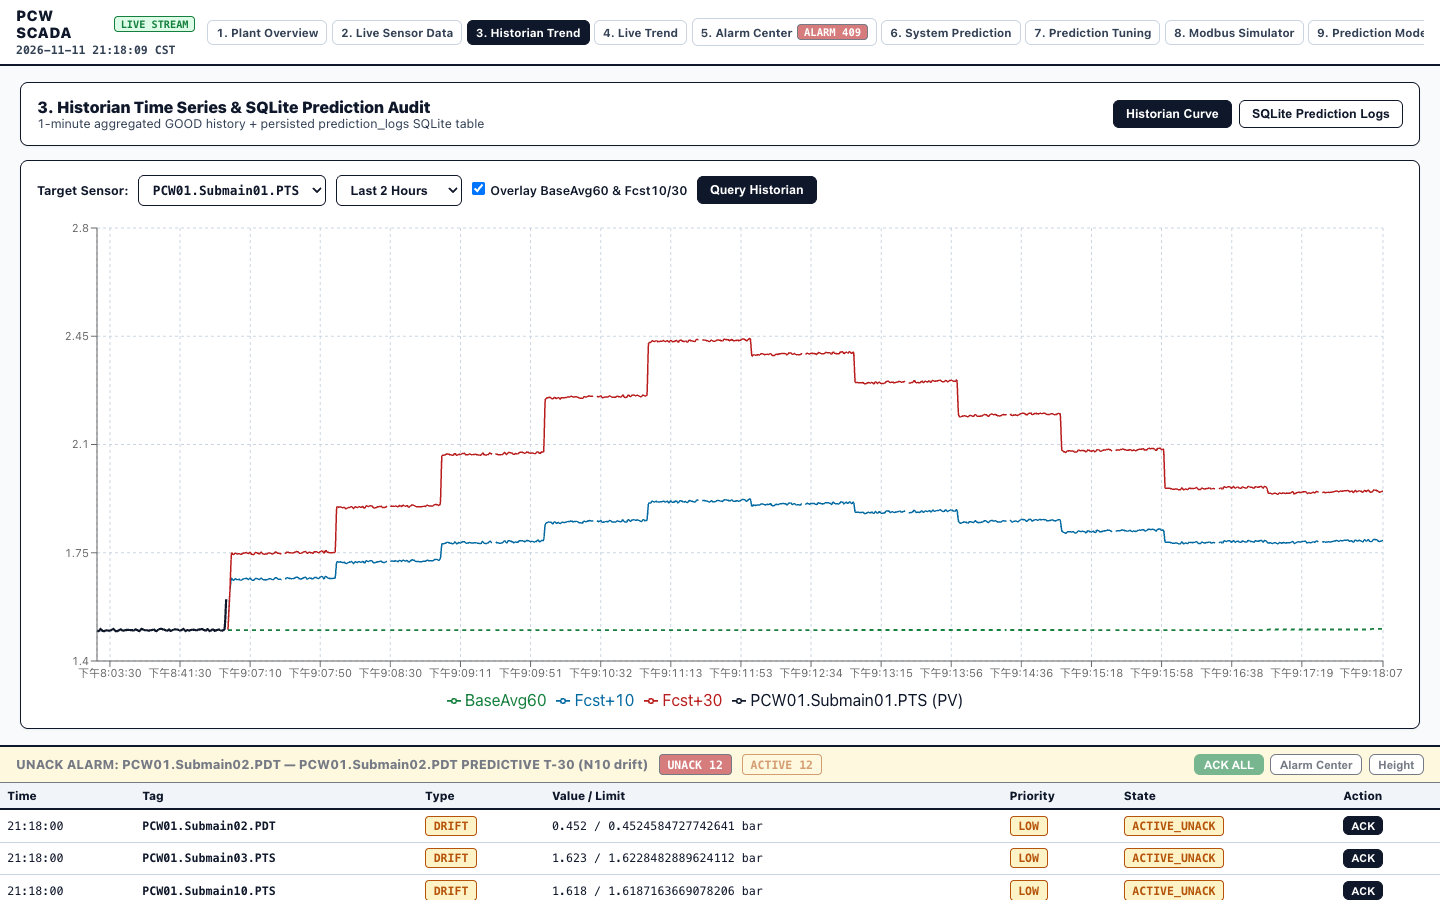
\includegraphics[width=0.92\textwidth,keepaspectratio]{picture/ui_local_historian.png}
    \caption{本機重構 v2.0 系統 11.35 分鐘真實時序 Historian 歷史曲線與外推預測軌跡截圖}
    \label{fig:ui_historian_new}
\end{figure}

% ============================================================
% 第五章 結論與未來展望
% ============================================================
\clearpage
\section{結論與未來展望}

\subsection{研究成果總結}
本研究針對半導體廠務 PCW 系統之早期壓力預警，完成了從數學定義、程式碼一致性重構、工業通訊整合到可重複實驗驗證之全鏈路工程實作：
\begin{enumerate}
    \item \textbf{嚴謹可驗證之統計預警演算法}：確立嚴格 Past-Only 70 分鐘因果視窗與 L1–L7 硬化規格，修正 $N_{10}>2.0$ 結構不可達盲區及 $>10$ 分鐘基準偏移失效率問題，並完成與 Excel 參考模型 100\% 一致性及 Python/TypeScript $<10^{-9}$ 跨語言對等驗證。
    \item \textbf{全廠 320 測點整合式系統重構}：實作具真實 Modbus/TCP 伺服器、SQLite 持久化歷史與逐測點預警執行紀錄、Pair Level 配對診斷與即時狀態同步之 Web SCADA 系統，徹底消除既有部署版本警報中心與預測頁面矛盾之缺陷。
    \item \textbf{誠實之公平基準與消融證據}：透過 3,840 場受控試驗完整揭露單點外推面對瞬態突波之誤報特性，並以消融實驗量化 2 分鐘前置確認對降低誤報率（$25.62\% \to 1.25\%\sim 6.88\%$）之顯著貢獻。
\end{enumerate}

\subsection{研究限制與未來工作}
本研究目前已完成本機與線上模擬器之長時序實測，但仍受限於缺乏真實晶圓廠多迴路歷史故障工單資料，且未經現場授權不得對實體 PLC 寫入參數。系統重構版雖已實作並開放 $\text{raw\_onset} \in \{1, 2\}$ 即時可調防抖參數，未來仍須透過廠內唯讀影子模式（Shadow Mode）收集跨維護週期實測數據並結合製程機台維修狀態遮罩（Layer 4 工況識別），以完成工業場域外部效度驗證。

% ==========================================
% 參考文獻
% ==========================================
\clearpage
\phantomsection
\addcontentsline{toc}{section}{參考文獻}
\bibliographystyle{IEEEtran}
\begin{thebibliography}{9}
\bibitem{isa1822016} International Society of Automation, \emph{ANSI/ISA-18.2-2016: Management of Alarm Systems for the Process Industries}, Research Triangle Park, NC, USA: ISA, 2016.
\bibitem{montgomery2020statistical} D. C. Montgomery, \emph{Introduction to Statistical Quality Control}, 8th ed. Hoboken, NJ, USA: John Wiley \& Sons, 2020.
\bibitem{roberts1959control} S. W. Roberts, ``Control chart tests based on geometric moving averages,'' \emph{Technometrics}, vol. 1, no. 3, pp. 239--250, 1959, doi: 10.1080/00401706.1959.10489860.
\bibitem{kaufman2012leakage} S. Kaufman, S. Rosset, C. Perlich, and O. Stitelman, ``Leakage in data mining: Formulation, detection, and avoidance,'' \emph{ACM Transactions on Knowledge Discovery from Data (TKDD)}, vol. 6, no. 4, pp. 1--21, 2012, doi: 10.1145/2382577.2382579.
\bibitem{darcy1857recherches} H. Darcy, ``Recherches exp{\'e}rimentales relatives au mouvement de l'eau dans les tuyaux,'' \emph{M{\'e}moires pr{\'e}sent{\'e}s par divers savants {\`a} l'Acad{\'e}mie des sciences de l'Institut imp{\'e}rial de France}, vol. 14, pp. 141--403, 1857.
\bibitem{colebrook1939turbulent} C. F. Colebrook, ``Turbulent flow in pipes, with particular reference to the transition region between the smooth and rough pipe laws,'' \emph{Journal of the Institution of Civil Engineers}, vol. 11, no. 4, pp. 133--156, 1939, doi: 10.1680/ijoti.1939.13150.
\bibitem{modbus2006spec} Modbus Organization, \emph{Modbus Messaging on TCP/IP Implementation Guide v1.0b}, Modbus Organization, Inc., 2006.
\end{thebibliography}

\end{doublespace}
\end{document}

